\chapter{城际高速铁路高密度运行建模与状态反馈控制}
\label{chap:ch2}

\section{引言}
\label{sec:ch2_intro}

随着我国城市群一体化进程加速，城际高速铁路（Intercity High-Speed Railway, IHSR）正朝着“公交化”运营模式发展，呈现出列车密度高、追踪间隔短、周期性运行强等典型特征。在此类高密度场景下，由客流波动引发的停站时间不确定性极易导致列车延误，并通过“前车晚点—后车等待”的连锁机制迅速传播，严重破坏运行图的稳定性与准点性。因此，构建能够精确刻画系统动态并支持实时调控的数学模型，是实现高效重调度的前提。

传统铁路调度方法多基于离散事件仿真或混合整数规划（MIP），其计算复杂度高，难以满足秒级实时决策需求。近年来，基于现代控制理论的状态空间方法因其低计算负担受到关注。然而，现有研究普遍建立在“单区间单车”（即列车数 $M$ 小于车站数 $N$）的理想假设之上，而实际城际高铁高峰时段常呈现“多车同区间”（$M > N$）的运行状态，使得传统模型失真。

针对上述挑战，本章以文献~\cite{Kang2024TITS}为基础，系统构建面向高密度城际铁路的离散时间状态空间模型，并设计相应的状态反馈控制器。主要贡献包括：（1）提出适用于 $M > N$ 场景的全局状态向量定义，显式刻画多列车在共享区间内的时空耦合关系；（2）建立包含客流-停站时间耦合效应的动态方程；（3）设计两类状态反馈控制器，分别面向“轻度延误恢复名义时刻表”与“重度延误维持均匀发车间隔”两种典型目标；（4）从理论上证明闭环系统的稳定性与收敛性。本章工作为后续鲁棒控制、迭代学习及模糊预测等高级策略奠定坚实的建模与控制基础。

\section{问题描述}
\label{problem}
为便于设计面向周期性时刻表运行的城际高速铁路（Intercity HSR）线路的实时自动重调度控制器，本节构建了列车到发时刻与客流耦合的状态空间模型。
首先在 \ref{2.A} 节引入环形线路模型，以表征双线城际高速铁路的运行特性，并考虑两种折返作业模式。
在 \ref{2.B} 节中，建立状态转移方程，用以刻画列车运行动态及其到发时刻与客流之间的相互作用。
城际高速铁路的状态空间模型在 \ref{2.C} 节中完成构建，并进一步分析当线路遭受初始延误时的延误传播特性与时刻表稳定性。

\subsection{交通运行描述}
\label{2.A}
为利用反馈控制设计方法求解双线城际高速铁路线路的实时自动重调度问题，本文引入环形线路模型。
考虑一条连接两座城市的双线城际高速铁路，共包含 $N/2$ 个物理车站，每个车站至少设有两个站台分别服务于上行与下行方向，如图~\ref{fig:change}(a) 所示。
为便于状态空间模型的构建，需区分上行与下行方向：将每个物理车站的上行与下行站台视为两个独立的车站，并以字母 $k$ 作为其编号。
因此，全线车站总数为 $N$，其中车站 $1,\cdots, N/2$ 对应上行方向，车站 $N/2+1, \cdots, N$ 对应下行方向。
共有 $M$ 列列车（$M > N$）沿该线路按序运行（包含两个方向），并在两个端点站进行折返后继续反向运行至另一端点站。
所有列车均在各站停车供乘客上下车。
本文考虑以地铁化模式运营的繁忙城际高速铁路线路，不允许列车越行。

\begin{figure}[htbp]
    \centering
    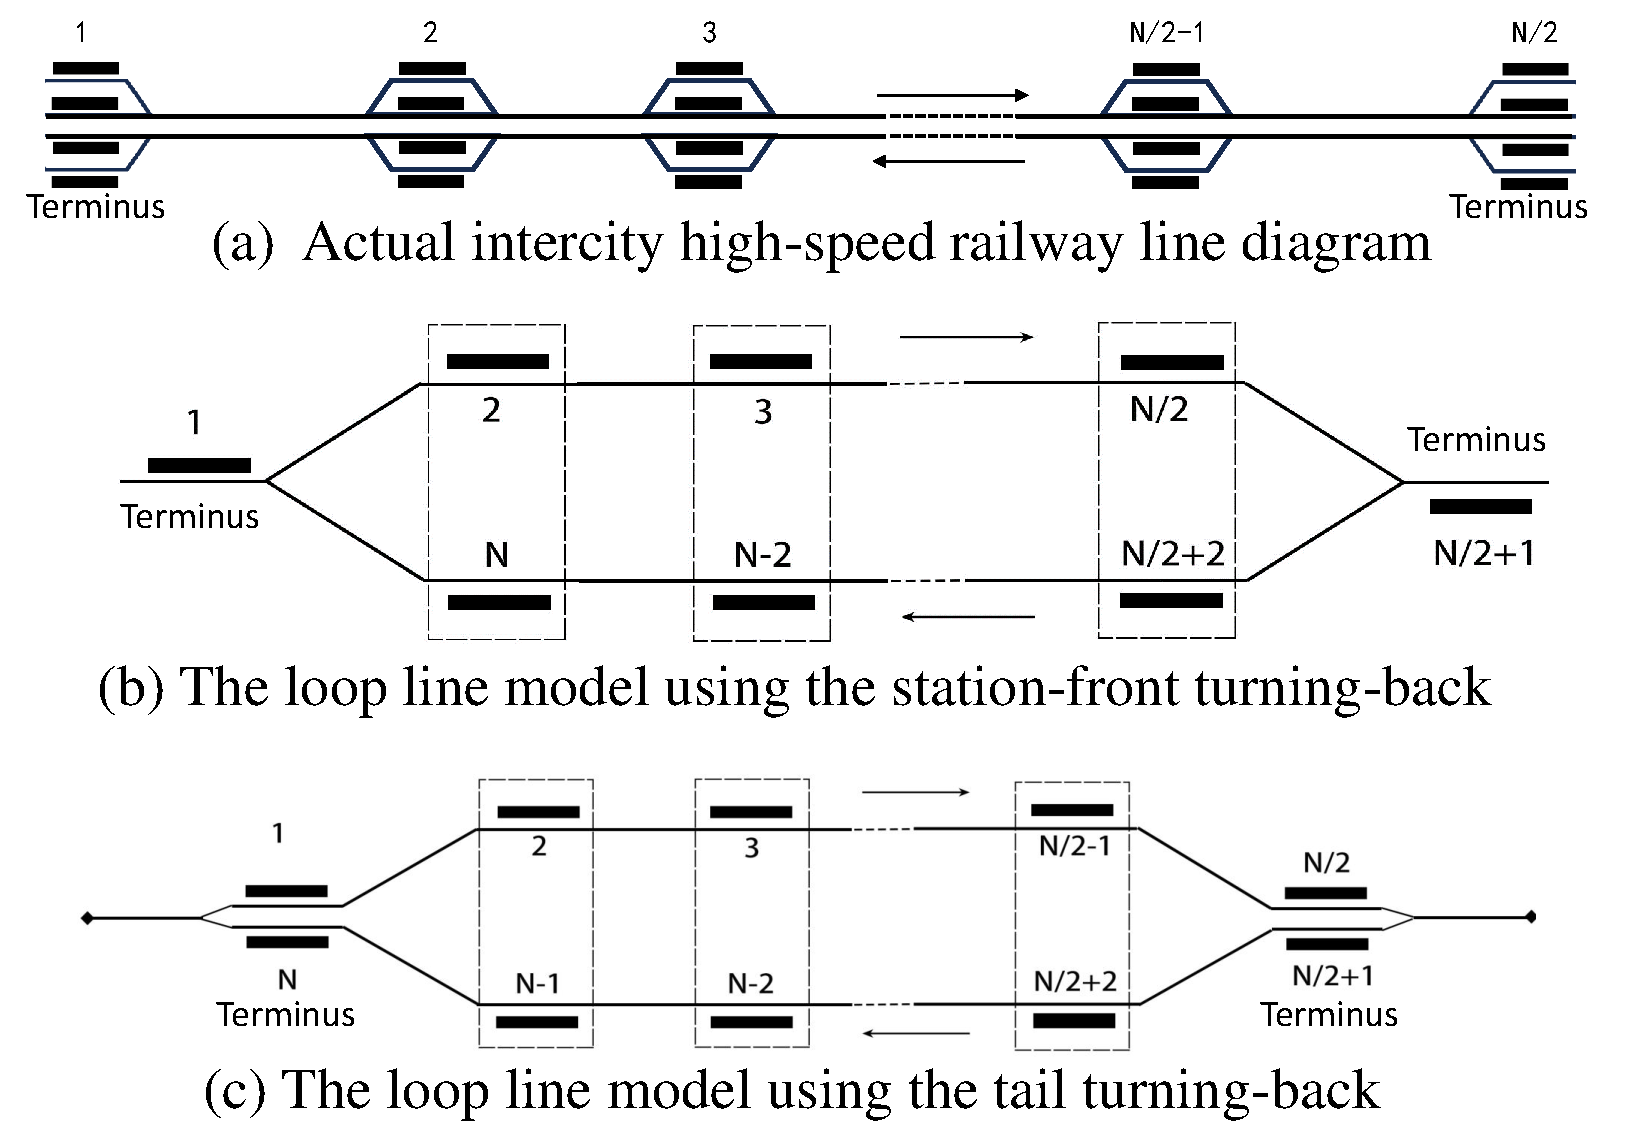
\includegraphics[width=\textwidth]{Img/Ch3/linechangestruct3.pdf} 
    \caption{双线城际高速铁路的两种单线环形线路模型}
    \label{fig:change}
\end{figure}

环形线路定义为一条包含 $N$ 个车站（编号为 $1$ 至 $N$）的闭合单线线路，其中车站 $N$ 与车站 $1$ 相连，且一组给定的列车（编号为 $1$ 至 $M$）沿该环形线路单向周期性运行。
在将双线城际高速铁路转换为单线环形线路模型时，根据端点站的折返作业模式不同，可引入两种环形线路模型：即图~\ref{fig:change}(b) 所示的**站前折返型环形线路**与图~\ref{fig:change}(c) 所示的**尾轨折返型环形线路**。

\textbf{站前折返（Station-front Turnaround）：} 当列车采用站前折返模式时，整体建模如图~\ref{fig:change}(b) 第二行所示。
由于上下客与折返作业均可在同一车站完成，因此该折返站可建模为单个车站。

\textbf{尾轨折返（Tail Turnaround）：} 当列车采用尾轨折返模式时，整体建模如图~\ref{fig:change}(c) 所示。
折返站首先使用一个车站供乘客下车，再使用另一个车站供乘客上车，因此可建模为两个车站。
折返时间可视为两站之间的运行时间。

如图~\ref{fig:change} 所示，无论城际高速铁路采用何种折返模式，均可建模为环形线路模型。
在任一环形线路模型中，各站所有列车的发车顺序均相同。
列车按顺时针顺序依次停靠各站，其序列为 $\{1,2, \cdots M, 1,2, \cdots M, 1,2 \cdots,\}$。
相应地，车站的有序序列为 $\{1,2, \cdots N, 1,2, \cdots N, 1,2 \cdots,\}$。

综上所述，一个包含 $N$ 个车站（$N$ 为偶数）的单线环形线路模型可有效表征包含 $N/2$ 个物理车站的双线城际高速铁路线路。
所提出的环形线路模型亦能更清晰地刻画双线城际高速铁路周期性运行中列车与车站之间的关联关系：
列车 $i$ 在车站 $k$ 的到发时刻演化，与其前行列车在同一车站 $k$ 的到发时刻以及其自身在前序车站 $\{k-1, k-2, \cdots \}$ 的历史到发时刻密切相关。

本文采用双下标符号体系标识与特定列车在特定车站相关的变量：上标 $i$ 表示列车编号，下标 $k$ 表示车站编号。
例如，$t_{k}^{i}$ 表示列车 $<i>$ 在车站 $<k>$ 的实际发车时刻。
为表征城际高速铁路的周期性运行特性，上述下标分别对 $M$ 和 $N$ 取模。
在此定义下，两列相邻列车可无失真地表示为 $i$ 与 $i+1$（列车 $M$ 后接列车 $1$），两座相邻车站可表示为 $k$ 与 $k+1$（车站 $N$ 后接车站 $1$）。

环形线路模型有助于构建交通动态的状态空间模型，并基于此设计反馈控制器。
本文所用关键变量列于表~\ref{table1}。

\begin{table}
    \centering
    \caption{变量定义}
    \label{table1}
    \begin{tabular}{cc}
        \hline
        变量 & 定义 \\
        \hline
        
        $t_{k}^{i}$ & 列车 $<i>$ 在车站 $k$ 的实际发车时刻 \\
        
        $r_{k}^{i}$ & 列车 $<i>$ 从车站 $k$ 至车站 $<k+1>$ 的实际运行时间 \\
        
        $s_{k}^{i}$ & 列车 $<i>$ 在车站 $k$ 的实际停站时间 \\
        
        $R_{k}$ & 从车站 $k$ 至车站 $<k+1>$ 的计划运行时间 \\
        
        $u_{k}^{i}$ & 对列车 $<i>$ 在区间 $k$ 至 $k+1$ 的运行时间施加的重调度调整量 \\
        
        $T_{k}^{i}$ & 列车 $<i>$ 在车站 $k$ 的计划发车时刻 \\
        
        ${w_1}_{k}^{i}$ & 运行时间的扰动项 \\
        
        ${w_2}_{k}^{i}$ & 停站时间的扰动项 \\
        
        $w_{k}^{i}$ & 扰动项之和 \\
        
        $H_{k}^{i}$ & 相邻列车之间的发车间隔 \\
        
        $c_{k}$ & 延误率，表示相邻列车发车间隔对停站时间的影响程度 \\
        
        $c$ & 延误率的常值 \\
        
        $S$ & 最小停站时间 \\
        
        $x_{k}^{i}$ & 实际发车时刻 $t_k^i$ 与计划发车时刻 $T_k^i$ 的偏差 \\
        
        $y_{k}^{i}$ & 列车 $<i>$ 与列车 $<i-1>$ 在车站 $<k>$ 的发车间隔相对于 $H$ 的偏差 \\
        
        $\delta u_{k}^{i}$ & 列车 $<i>$ 与 $i-1$ 在车站 $<k>$ 的重调度调整量 $u_k^i$ 与 $u_k^{i-1}$ 的偏差 \\
        
        $\delta w_{k}^{i}$ & 列车 $<i>$ 与 $i-1$ 在车站 $<k>$ 的扰动项 $w_k^i$ 与 $w_k^{i-1}$ 的偏差 \\
        
        \hline
    \end{tabular}
\end{table}

\subsection{列车交通流模型}
\label{2.B}
文献~\cite{b22} 提出了一种列车交通流模型，并被后续研究~\cite{b21} 所采用，但其基于一个不切实际的假设：列车数与车站数相等（即每区间仅有一列车）。
本文将其扩展至允许列车数大于车站数的情形（即区间内存在多列车），这更符合城际高速铁路的实际运行场景。
列车 $<i>$ 从车站 $<k+1>$ 的发车时刻可表示为
\begin{equation}
    t_{k+1}^{i}=t_{k}^{i}+r_{k}^{i}+s_{k+1}^{i} 
    \label{equ:equ1}
\end{equation}
其中 $r_{k}^{i}$ 为列车 $<i>$ 从车站 $k$ 至车站 $k+1$ 的实际运行时间，$s_{k+1}^{i}$ 为列车 $<i>$ 在车站 $<k+1>$ 的停站时间。
根据假设 1 与 2，实际运行时间为
\begin{equation}
    r_{k}^{i}=R_{k}+u_{k}^{i}+{w_1}_{k}^{i}
    \label{equ:equ2}
\end{equation}
其中 $R_{k}$ 为从车站 $<k>$ 至车站 $<k+1>$ 的计划运行时间，
$u_{k}^{i}$ 表示重调度过程中对列车 $<i>$ 在区间 $<k>$ 至 $<k+1>$ 运行时间的调整量。
${w_1}_{k}^{i}$ 为运行时间的不确定性项，用于建模由突发事件（如极端天气导致的临时限速、设备或基础设施故障）或司机行为差异等引起的计划时刻表偏差。

停站时间可建模为
\begin{equation}
    s_{k+1}^{i}=S+c_{k+1}(t_{k+1}^{i}-t_{k+1}^{i-1})+{w_2}_{k+1}^{i}
    \label{equ:equ3}
\end{equation}
其中 $S$ 为列车在车站的最小停站时间，$c_k$ 为客流引起的延误率，表示相邻列车发车间隔对停站时间的影响程度~\cite{b11}。
这意味着，发车间隔越大，车站积压乘客越多，所需停站时间越长以容纳更多上车乘客。
${w_2}_{k+1}^{i}$ 为停站时间的干扰项。
为便于描述，将干扰项合并为
\begin{equation}
    w_{k}^{i}={w_1}_{k}^{i}+{w_2}_{k+1}^{i}
    \label{equ:equ4}
\end{equation}
其中 $w_{k}^{i}$ 为总干扰项。
根据式~(\ref{equ:equ2}) 与 (\ref{equ:equ3})，将变量 $r_k^i$ 与 $s_k^i$ 代入式~(\ref{equ:equ1})，并依据式~(\ref{equ:equ4}) 合并 ${w_1}_{k}^{i}$ 与 ${w_2}_{k+1}^{i}$，可得
\begin{equation}		
    (1-c_{k+1})t_{k+1}^{i}=t_{k}^{i}-c_{k+1}t_{k+1}^{i-1}+S+R_{k}+u_{k}^{i}+w_{k}^{i}
    \label{equ:equ5}
\end{equation}
式~(\ref{equ:equ5}) 可重写为：
\begin{equation*}
    t_{k+1}^i=t_k^i-c_{k+1}\left(t_{k+1}^{i-1}-t_{k+1}^i\right)+S+R_k+u_k^i+w_k^i
\end{equation*}
该方程刻画了列车 $<i>$ 在车站 $<k+1>$ 的发车时刻 $t_{k+1}^i$ 与其在前序车站 $<k>$ 的发车时刻 $t_k^i$ 以及客流（由延误率 $c_{k+1}$ 与相邻列车 $<i-1>$ 与 $<i>$ 的发车间隔 $t_{k+1}^{i-1}- t_{k+1}^i$ 表征）之间的关系。

为满足防撞安全要求，允许的控制动作 $u_{k}^{i}$ 与干扰 $w_{k}^{i}$ 均为有界量。
式~(\ref{equ:equ5}) 给出了与两列相邻列车及两座相邻车站相关的局部交通行为描述。

\textbf{计划时刻表（Nominal timetable）：}
计划时刻表是定义列车在沿线各站计划到发时刻的基础时刻表，实际运行以此为基准进行比对。
令 $T_{k}^{i}$ 表示列车 $i$ 在车站 $k$ 的计划发车时刻，$H_{k}^{i}$ 表示车站 $k$ 处相邻列车的计划发车间隔，则有
\begin{equation}
    H_{k}^{i}=T_{k}^{i+1}-T_{k}^{i}  
    \label{equ:equ6}
\end{equation}
同一位置点连续通过列车的时间间隔亦称为\emph{发车间隔（Headway）}，式~(\ref{equ:equ6}) 中的 $H_k^i$ 即为发车发车间隔，本质上反映了列车之间的间距。

常规周期性时刻表具有规则的发车间隔特征。例如，每 5 分钟有一列车到发，即要求相邻列车间的发车间隔 $H_k^i$ 尽可能恒定。
考虑一个包含 $M$ 列列车的城际高速铁路环形线路模型，若列车沿全线均匀分布以提供周期为 $H$ 的规则服务，则列车完成整圈运行的总时间等于 $H$ 与列车数 $M$ 的乘积。
同时，该总运行时间亦等于所有 $N$ 个区间运行时间与各站停站时间之和。
现有研究中，通常假设各站延误率相同（$c_{k}=c$），即
\begin{equation}
    MH=N[S+cH]+\sum_{k=1}^NR_{k}
    \label{equ:equ7}
\end{equation}

当发车间隔趋于规则时，发车间隔规则性得以提升，同时乘客平均等待时间降低~\cite{b23}。
在无延误或交通中断的正常运行状态下，不确定延误 $\omega_k^i=0$，且无需调整运行时间，故重调度动作 $u_k^i = 0$。
因此，在无延误的正常运行中，发车时刻 $T_k^i$ 的演化可由通用模型~(\ref{equ:equ5}) 简化得到：
\begin{equation}
    T_{k+1}^{i}=T_{k}^{i}+cH+S+R_{k}
    \label{equ:equ8}
\end{equation}
式~(\ref{equ:equ7}) 实际上描述了计划时刻表中的发车时刻演化规律。

实践中，突发事件可能导致列车实际到发时刻偏离计划时刻表。
令 $x_{k}^{i}$ 表示实际发车时刻 $t_k^i$ 与计划发车时刻 $T_{k}^{i}$ 的偏差（亦称\emph{发车延误}），即
\begin{equation}
    x_{k}^{i}=t_{k}^{i}-T_{k}^{i}  
    \label{equ:equ9}
\end{equation}

根据式~(\ref{equ:equ5})、(\ref{equ:equ6})、(\ref{equ:equ8}) 与 (\ref{equ:equ9})，
将式~(\ref{equ:equ8}) 中的 $H$ 用式~(\ref{equ:equ6}) 替换，再将替换后的式子与式~(\ref{equ:equ5}) 相减，并利用式~(\ref{equ:equ9}) 替换 $t_{k}^{i}-T_{k}^{i}$，可得发车延误的演化方程：
\begin{equation}
    (1-c)x_{k+1}^{i}+cx_{k+1}^{i-1}=x_{k}^{i}+u_{k}^{i}+w_{k}^{i},k\geq0,i\geq1
    \label{equ:equ10}
\end{equation}
该式可进一步重写为：
\begin{equation*}
    x_{k+1}^i=x_k^i-c\left(x_{k+1}^{i-1}-x_{k+1}^i\right)+u_k^i+w_k^i
\end{equation*}
显然，该方程刻画了列车 $<i>$ 在车站 $<k+1>$ 的发车延误 $x_k^i$、其在前序车站 $<k>$ 的发车延误 $x_k^i$ 以及客流之间的关系。
式~(\ref{equ:equ7}) 定义了计划时刻表（其中 $H$ 为计划间隔），而扰动方程~(\ref{equ:equ10}) 同样适用于环形线路。

\subsection{城际高速铁路的状态空间模型}
\label{2.C}
本节构建表征所有列车在所有车站发车时刻演化的数学模型。
传统铁路发车时刻状态空间模型通常假设每区间仅允许一列车运行~\cite{b21}，本文对其进行了扩展，使模型更具现实性与实用性。

为便于环形线路状态空间模型的扩展，引入两个参数化变换矩阵 $D_1(a,b)$ 与 $D_2(a)$。
$D_{1}(a,b)\in \mathbb{R}^{M \times N}$ 定义为

\begin{equation*}
    D_{1}(a,b)=
    \begin{array}{ccccccccc}
        \setlength{\arraycolsep}{1mm}
        \left[
        \begin{array}{ccc|cccc}
            0&1& & & & & 0\\
            0&\ddots&\ddots & & & & \\
            & &0&1& & & \\ 
            \cline{1-7}
            0& & &a&b& & \\
            & & & &\ddots&\ddots& \\
            & & & & & a&b\\
            b& & & & & &a\\
        \end{array}
        \right]
        & 
        \begin{array}{c}
            \left.\rule{0mm}{3.5mm}\right\}M-N  \\ \hfill
            \\
            \\
            \left.\rule{0mm}{3.5mm}\right\}N \hfill
            \\
        \end{array} \\
        \begin{array}{cc}
            \underbrace{\rule{14mm}{0mm}}_{M-N} &  
            \underbrace{\rule{18mm}{0mm}}_{N}
        \end{array}
    \end{array}
\end{equation*}
其中参数 $a$ 与 $b$ 用于表征列车延误的演化特性。

变换矩阵 $D_{2}(a)\in \mathbb{R}^{N \times N}$ 定义为
\begin{equation*}
    D_{2}(a)=
    \begin{array}{cccccc}
        \setlength{\arraycolsep}{1.5mm}
        \left[
        \begin{array}{ccc}
            & 0&  \\
            \cline{1-3}
            a& &0\\ 
            &\ddots & \\
            0& &a\\
            
        \end{array}
        \right]
        &  
        \begin{array}{c}
            \left.\rule{0mm}{2mm}\right\}M-N \\ 
            \\
            \left.\rule{0mm}{4mm}\right\}N \hfill\\
            \\
        \end{array}
    \end{array}
\end{equation*}

对于包含 $M$ 列列车与 $N$ 个车站（$N > M$）的环形线路模型，引入 $M$ 维\emph{状态向量} $X_k^i$ 以表征所有 $M$ 列列车的延误：
\begin{gather}
    X_{k}^{i}=\underbrace{\left[x_{k}^{i-M} x_{k}^{i-M+1} \cdots x_{k}^{i-N-1}\right.}_{M-N} \underbrace{x_{k}^{i-N} x_{k-1}^{i-N+1} \cdots x_{k-N+1}^{i-1}}_{N}]^{\top}  
    \label{equ:equ11:state}
\end{gather}
状态向量 $X_k^i$ 以任意车站 $<k>$ 与任意列车 $<i>$ 为参考点进行定义。
值得注意的是，在环形模型中，列车编号与车站编号分别以 $M$ 和 $N$ 为模呈循环特性，因此参考点的选择具有任意性。
状态向量 $X_k^i$ 由两部分组成：

1) \textbf{车站 $k$ 处的延误：} $X_k^i$ 的前 $M-N$ 项为车站 $<k>$ 处 $M-N$ 列相邻列车（列车 $<i - M>$ 至 $<i - N - 1>$）的延误；

2) \textbf{前序列车在前序车站的延误：} 后 $N$ 项为前序 $N$ 列列车（列车 $<i-N>$ 至 $<i-1>$）在前序车站（从车站 $k$ 至 $k-N+1$）的延误。
这些项的特征是其上标与下标之和为同一常值（分别对 $M$ 和 $N$ 取模），例如上标 $i-N$ + 下标 $k$ = $i+k-N$，上标 $i-1$ + 下标 $k-N+1$ = $i+k-N$，依此类推。

类似地，定义 $N$ 维控制向量 $U_{k}^{i}$ 与 $N$ 维干扰向量 $W_{k}^{i}$ 如下：
\begin{gather}
    U_{k}^{i}={[\underbrace{u_{k-1}^{i-N+1} u_{k-2}^{i-N+2} \cdots u_{k-N}^{i}}_{N}}]^{\top} 
    \label{equ:equ12}
\end{gather}

\begin{gather}
    W_{k}^{i}=\underbrace{\left[w_{k-1}^{i-N+1} w_{k-2}^{i-N+2} \cdots w_{k-N}^{i}\right.}_{N}]^{\top} 
    \label{equ:equ13}
\end{gather}
控制向量与干扰向量作用于 $M$ 列列车中的 $N$ 列子集。
根据 $X_k^i$、$U_k^i$ 与 $W_k^i$ 的定义，可由单车模型~(\ref{equ:equ10}) 推导出如下多列车状态空间模型：
\begin{equation} 
    X_{k}^{i+1}=A_{L} X_{k}^{i}+B_{L}\left[U_{k}^{i}+W_{k}^{i}\right], \quad k \in\{1,2, \cdots,N\}
    \label{equ:equ14:model}
\end{equation}
\begin{equation*}
    A_{L}=D_{1}\left(\frac{-c}{1-c}, \frac{1}{1-c}\right) \quad B_{L}=D_{2}\left(\frac{-c}{1-c}\right)
\end{equation*}

\begin{figure}[htbp]
    \centering
    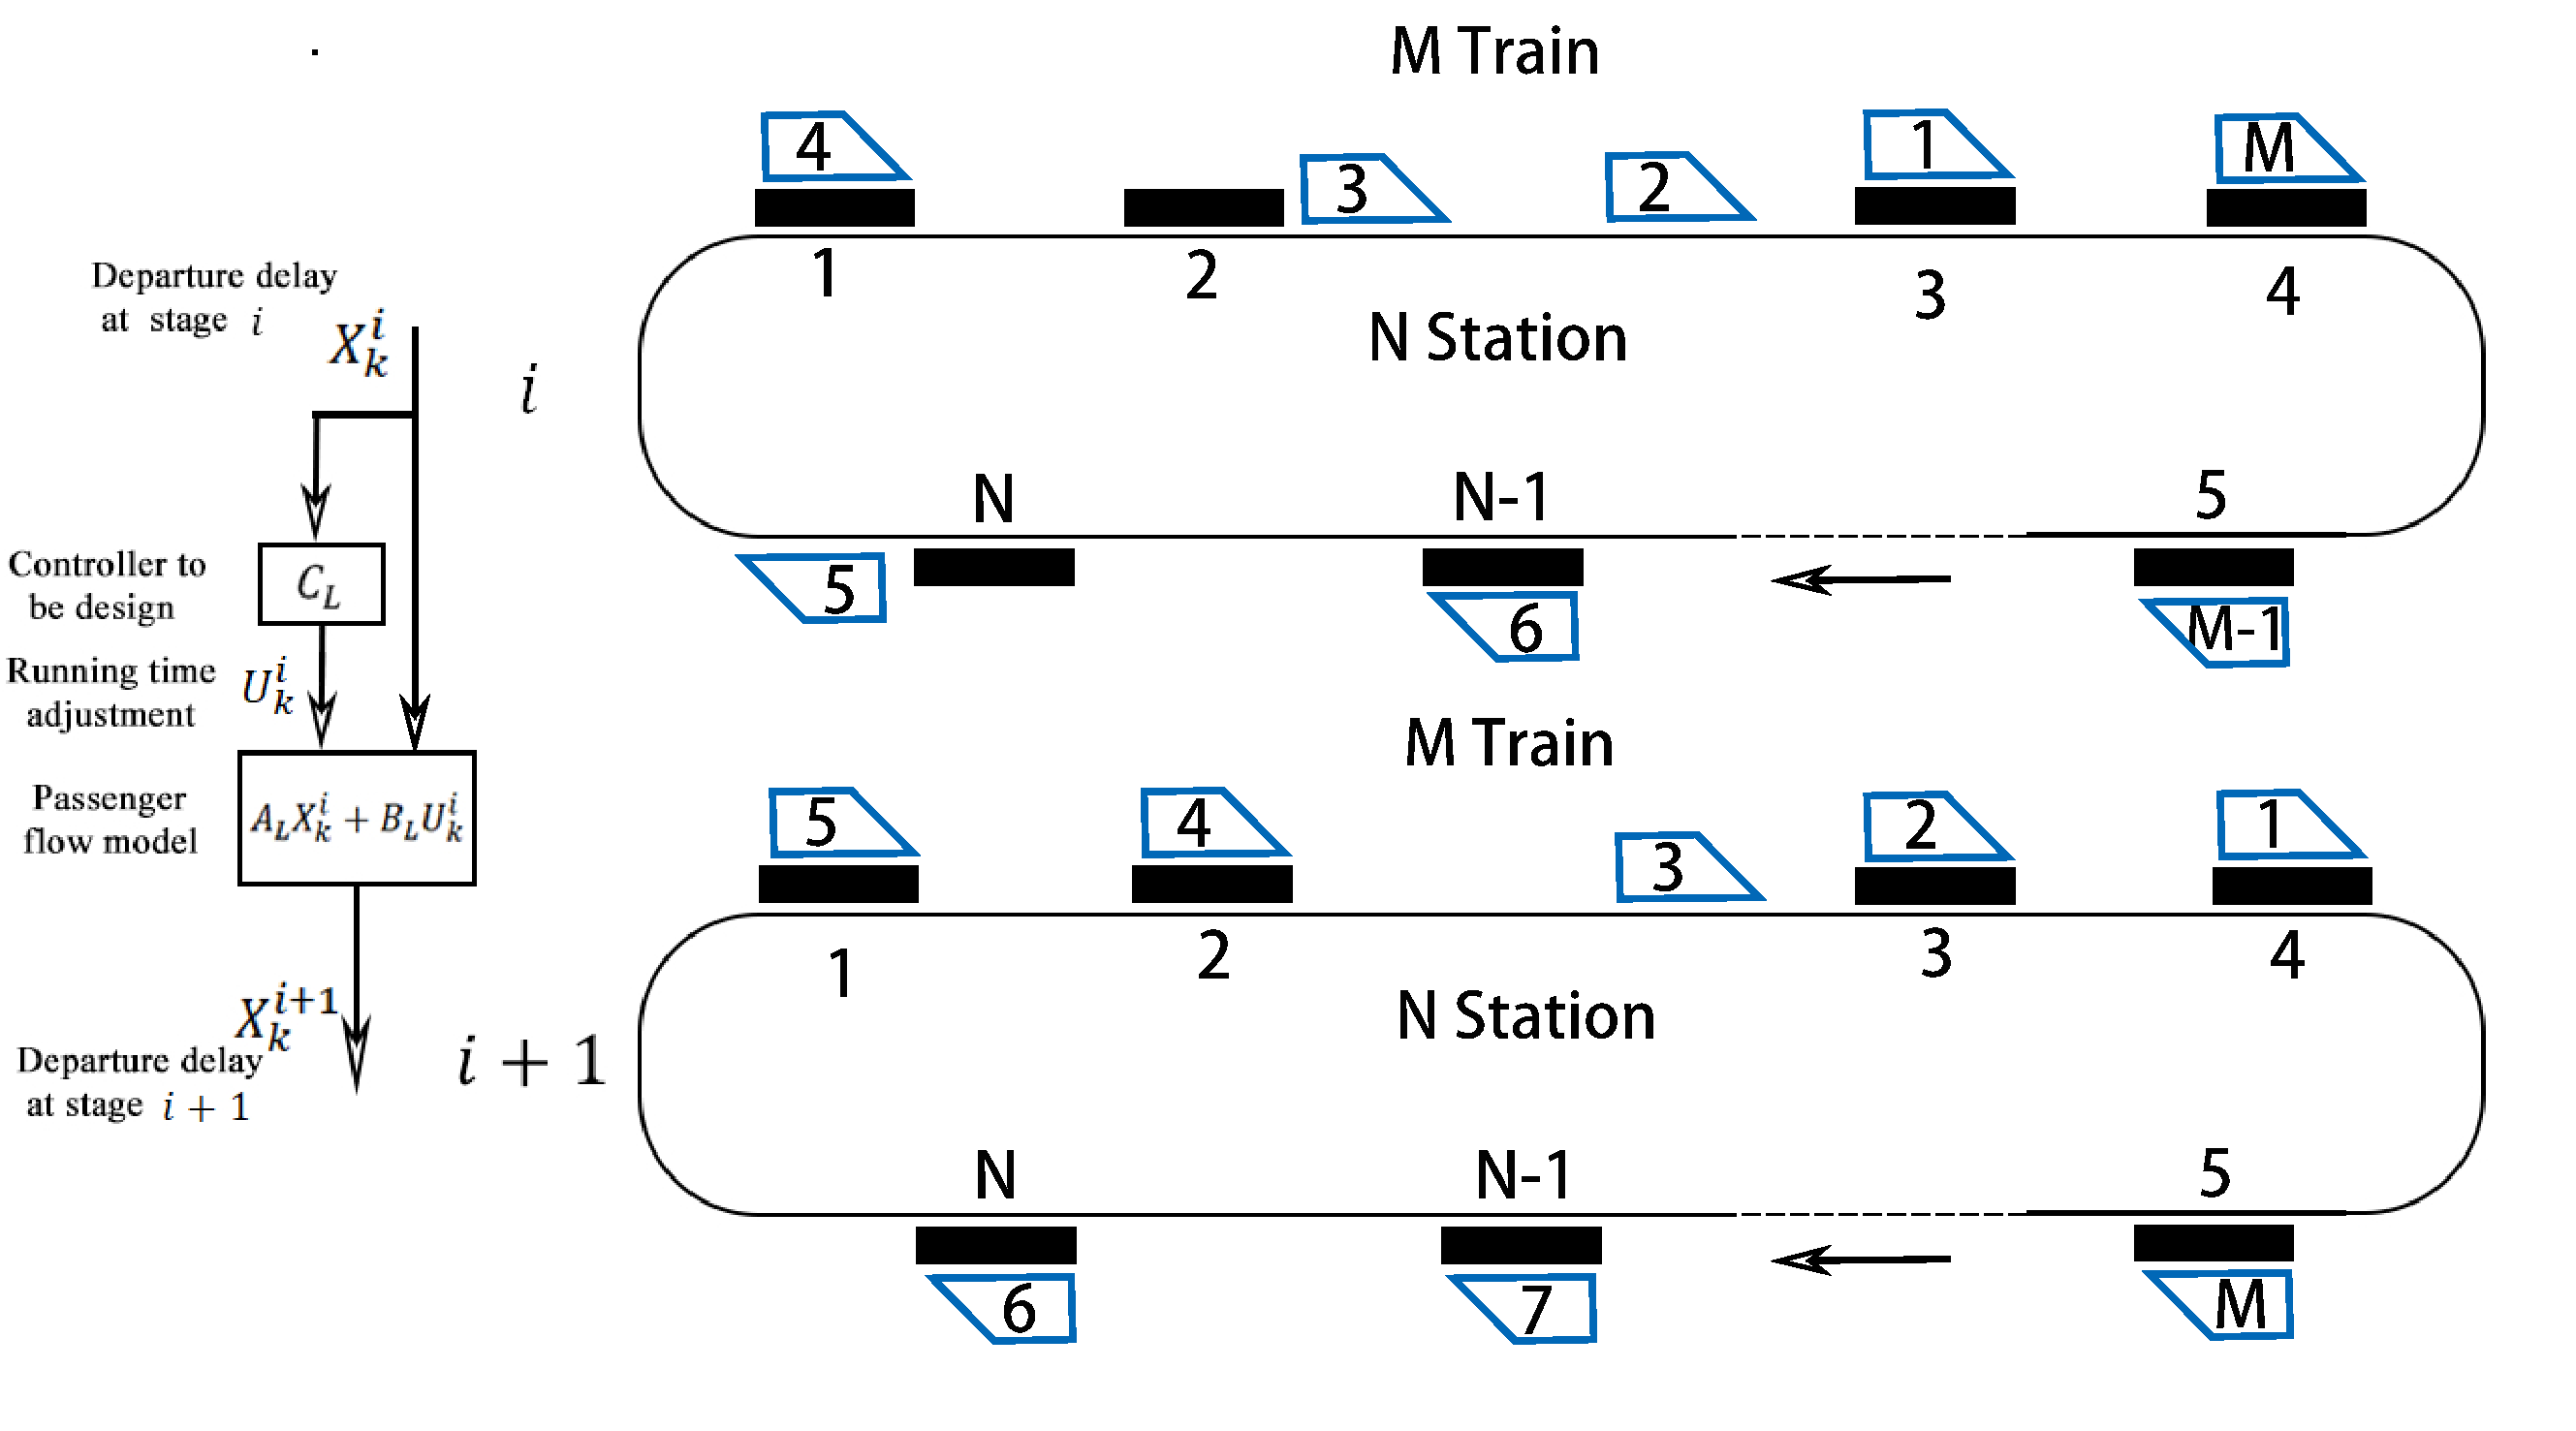
\includegraphics[width=\textwidth]{Img/Ch3/linechange.pdf} 
    \caption{列车运行演化示意图}
    \label{fig3}  
\end{figure}

所提模型的概念如图~\ref{fig3} 所示，描绘了状态向量从阶段 $i$ 至阶段 $i+1$ 的转移过程。
该模型为事件驱动型，其中事件定义为每站均有列车到达。
阶段 $i$ 表示列车 $\{<i-N>, <i-N+1>, \cdots, <i-1>\}$ 从车站 $\{k, k-1, \cdots, k-N+1\}$ 发车，其余列车 $\{<i-M>, <i-M+1>, \cdots, <i-N-1>\}$ 从车站 $k$ 发车（$<>$ 表示对 $M$ 取模）。
阶段 $i+1$ 表示这些列车到达其下一站。
值得注意的是，实践中无法安排每列车的到达时刻完全同步，各列车的到达事件可能发生在不同时刻。
因此，在阶段 $i$，若以列车 $<i-N>$ 从车站 $k$ 发车的时刻为参考时间，则其他列车从其计划车站的发车时刻可确定如下：
若某列车的发车事件早于列车 $<i-N>$，则采用其实际发车时刻（及发车延误）；
若该列车尚未从其计划车站发车，则采用预测发车时刻（及预测发车延误）。
车站 $k$ 的选择可在 $k \in\{1,2, \cdots, N\}$ 范围内任意选取。
鉴于城际高速铁路采用周期性时刻表且发车间隔规则，合理选择参考列车与车站可使状态向量 $X_{k}^{i}$ 的大部分分量已知，仅需对少数分量进行发车时刻预测。
文献中已提出多种此类发车时刻估计算法~\cite{b22}。

如图~\ref{fig3} 的示例所示，所提模型允许多列车存在于车站之间。

为便于城际高速铁路运行与重调度控制器的稳定性分析，本文采用一种稳定性指标，称为\emph{运行质量指数（Operation Quality Index, OQI）}：
\begin{equation}
    \prod_{j}=\frac{1}{N} \sum_{k=1}^{N}\left(x_{k}^{j-k}\right)^{2}
    \label{equ:equ15}
\end{equation}
该指标由 $N$ 列列车（从列车 $<j-1>$ 至 $<j-N>$）在 $N$ 个车站的发车延误平方平均值构成。
注意，此处仅考虑 $M$ 列列车中的 $N$ 列，整数 $j$ 反映了 OQI 指标中所考虑的具体车站与列车延误。
$j$ 的选择通常与某一阶段关联，并对应特定的“列车-车站”模式（即哪些列车在哪些车站的延误被考虑）。
例如，在图~\ref{fig3} 的阶段 $i$，若列车 4 位于车站 $k=1$，可选择 $j=5$，则后续项依次为列车 3 在车站 2 的延误，依此类推。
此时，OQI 仅考虑列车 $\{4, 3,2,1,M, M-1,\cdots, M-N+4\}$ 在车站 $\{1, \cdots, N\}$ 的延误。
值得注意的是，由于区间内存在多列车（如列车 3 与 2 位于车站 2 至 3 的区间内），下一项即为列车 2 在车站 3 的延误 $x_3^{5-3}$。

在无交通中断的正常运行状态下，所有列车准点运行，OQI~(\ref{equ:equ15}) 为 0。
OQI 值 $\prod_{j}$ 随列车到达下一站而演化（即环形线路模型进入下一阶段）。
由于运行的周期性及编号的循环特性（取模运算），阶段 $i$ 的 OQI（对应 $j$）与阶段 $i+M$ 的 OQI（对应 $j+M$）具有相同的“列车-车站”模式（因所有列车已完成一圈运行，运行模式重复），但 OQI 值通常不同。
OQI 的变化量为
\begin{equation*}
    \prod_{j+M}-\prod_{j}=\frac{1}{N} \sum_{i=1}^{N}\left[\left\|X_{k}^{i+1}\right\|^{2}-\left\|X_{k}^{i}\right\|^{2}\right]
\end{equation*}

借鉴控制理论中的自由运行系统概念，本文定义城际高速铁路系统的自由响应为：系统在无任何外部干预或控制输入（即无干扰、无重调度）情况下，仅依据其内部动态演化的运行行为。
状态空间环形线路模型~(\ref{equ:equ14:model}) 的自由响应为
\begin{equation}
    X_k^{i+1} = A_LX_k^i
    \label{equ:equ18}
\end{equation}
其中重调度动作 $U_k^i =0$，外部干扰 $W_k^i=0$。
关于系统稳定性，提出以下定理。

\textbf{定理 1：} 对于 $c >0$，当城际高速铁路线路系统~(\ref{equ:equ14:model}) 处于平衡状态时，若其遭受有界外部干扰 $W_k^i \neq 0$，则存在整数 $k_0 \in \{1,\cdots, M\}$ 与 $l_0 \in \{1,\cdots, M\}$，使得对任意 $\forall k \geq k_{0}, \forall l \geq l_{0}$ 及所有 $\forall i(i=1, \cdots, M), \forall j(j=1, \cdots, N)$，满足：

1) $\left\|X_{k}^{i+1}\right\|>\left\|X_{k}^{i}\right\|$

2) $\prod_{j+(l+1)\ast M}>\prod_{k+l\ast M}$

\textbf{证明：} 首先，任何与式~(\ref{equ:equ11:state}) 兼容的实际扰动仅影响状态向量的后 $N$ 个分量。

其次，为分析 $A_L$ 的特征值分布，考虑第一个向量 $Q_{1}\left(\in \mathbb{R}^{N}\right)$
\begin{equation*}
    \begin{aligned}
        Q_{1}=\left[\begin{array}{l}
            P \\
            0
        \end{array}\right] \text { 其中 } P=\left(p_{1}, p_{2}, \cdots, p_{M-N}\right)^{\top} & \in \mathbb{R}^{M-N}, V \neq 0
    \end{aligned}
\end{equation*}
显然可得 $\left\|A_{L} Q_{1}\right\| \leq\left\|Q_{1}\right\|$，若 $p_1 \neq 0$，则 $\left\|A_{L} Q_{1}\right\| <\left\|Q_{1}\right\|$。

考虑第二个向量 $Q_{2}\left(\in \mathbb{R}^{N}\right)$
\begin{equation*}
    \begin{aligned}
        &Q_{2}=\left[\begin{array}{l}
            0 \\
            P
        \end{array}\right] \quad \text { 其中 } \quad P=\left(p_{1}, p_{2}, \cdots, p_{N}\right)^{\top} \in \mathbb{R}^{N}, \quad P \neq 0 \\
        &\begin{aligned}
            \left\|A_{L} Q_{2}\right\|^{2} &=q_{1}^{2}+\left\|A_{22} \cdot P\right\|^{2} \geq\left\|A_{22} P\right\|^{2}>\|P\|^{2} \\
            &=\left\|Q_{2}\right\|^{2}
        \end{aligned}
    \end{aligned}
\end{equation*}
其中
\begin{equation*}
    A_{22}=\left[\begin{array}{cccc}
        -c /(1-c) & 1 /(1-c) & 0 & \\
        & -c /(1-c) & \ddots & \\
        & & \ddots & 1 /(1-c) \\
        0 & & & -c /(1-c)
    \end{array}\right]
\end{equation*}

综合上述两种情形，矩阵 $A_L$ 至少有一个特征值位于单位圆内，一个特征值位于单位圆外。
考虑一个通过扰动平衡状态得到的状态向量 $X_0$（扰动形式与式~(\ref{equ:equ11:state}) 兼容），可表示为
\begin{equation}
    X_{0}=\alpha_{0} \lambda_0+\sum_{i=1}^{n_{1}} \alpha_{i} \lambda_i+\sum_{k=1}^{n_{2}} \beta_{k} \theta_k \quad \text { 其中 } \quad \alpha_{i}, \beta_{k} \in \mathbb{R}
\end{equation}
其中 $\lambda_0$ 为特征值 1 对应的特征向量（$\lambda_{0}=[1,\cdots,1]^{\top}$），
$\lambda_i\left(i=1,\cdots,n_1\right)$ 为稳定特征值对应的特征向量，
$\theta_i\left(i=1,\cdots,n_1\right)$ 为不稳定特征值对应的特征向量。
由于扰动形式与 $Q_2$ 类似，至少有一个系数 $\beta_{k}$ 非零。

如定理 1 所证，在客流延误率 $c=0$ 的特殊情形下，$A_L$ 的特征值为 0 与 1，且其几何重数等于代数重数，表明自由运行系统稳定。
然而，由于存在特征值 1，系统并非渐近稳定，这意味着在有界外部干扰作用下，系统响应无法保证有界。
换言之，当外部干扰引发初始延误时，时刻表可能无法恢复。
对于 $c>0$，系统存在一个特征值 1，其对应特征向量为 $[1 \cdots 1]^{\top}$。
当所有偏差具有相同值时，该平衡点为不稳定平衡点：任何扰动均将导致 OQI $\prod_j$ 发散至无穷大。

因此，在无重调度控制输入的情况下，采用周期性计划时刻表运行的城际高速铁路线路的延误将持续累积。
定理 1 揭示了城际高速铁路线路在外部干扰下的天然不稳定性，从而凸显了交通控制策略的必要性。
如前所述，对于以地铁化周期模式运营的城际高速铁路，存在两类重调度目标：
轻度延误时恢复计划时刻表，重度延误时维持规则发车间隔。
针对这两种场景，将分别设计两类状态反馈控制器以实现实时自动重调度。

\section{名义时刻表恢复的反馈控制器设计}
\label{sec:guidelines}
本节针对周期性线路结构，设计一种专用控制器。我们的目标是在维持运行稳定性的同时，最小化对时间裕度的需求以及在运列车总数。为此，我们设计了一个控制性能指标，并开发了一个能够有效实现上述目标的稳定控制器。

给定当前晚点状态 $X_k^i$（假设状态向量 $X_k^i$ 表示所有列车的当前晚点状态），令 $J_{1}^{k}$ 表示名义时刻表恢复的目标函数，$J_{1}^{k}$ 可定义为最小化晚点状态 $X_k^i$。同时，考虑到“随到随走”型乘客期望获得规律的服务，即候车时间不宜过长且车站不发生过度拥挤，因此在恢复时刻表的过程中，也应尽可能保持发车间隔的规律性。

性能指标定义如下：
\begin{scriptsize}
	\begin{gather}
		J_{1}^{k}=\left(X_{k}^{i+1}\right)^{T} P\left(X_{k}^{i+1}\right)+\left(X_{k}^{i+1}-S_{M} X_{k}^{i}\right)^{T} Q\left(X_{k}^{i+1}-S_{M} X_{k}^{i}\right) \notag\\
		+\left(U_{k}^{i}\right)^{T} U_{k}^{i}
		\label{equ:equ18:opti1}
	\end{gather}
\end{scriptsize}
其中权重矩阵为
\begin{align*}
	P &= \text{diag}(0,\ldots,0,p,\ldots,p) \\
	Q &= \text{diag}(0,\ldots,0,q,\ldots,q) \\
	S_{M} &= \begin{bmatrix}
		0 & 1 & & 0 \\
		& \ddots & \ddots & \\
		0 & & & 1 \\
		1 & & & 0
	\end{bmatrix}
\end{align*}
$P$ 和 $Q$ 均为 $N$ 维对角矩阵，其前 $N-M$ 个元素为 0，其余元素分别为两个非负参数 $p$ 和 $q$。$S_M$ 为 $M \times M$ 维置换矩阵。$P$ 与 $Q$ 用于调节在延误恢复过程中对发车间隔规律性的保持程度。

目标函数 $J_1^k$ 的第一项惩罚 $N$ 列列车的晚点状态，第二项惩罚相邻列车之间发车间隔相对于名义值 $H$ 的偏差，第三项则对控制量进行惩罚，以避免控制器输出过大。

\textbf{注 1：} 目标函数 (\ref{equ:equ18:opti1}) 中的第二项与第 \ref{section:4} 节所提出的保持规律发车间隔的方法不同。此处包含 $X_k^i$ 的项仍需考虑名义时刻表，并非单纯追求发车间隔的规律性。而第 \ref{section:4} 节所设计的模型与目标函数仅关注发车间隔规律性，未考虑名义时刻表。

现提出如下名义时刻表恢复的反馈控制器。在满足线性约束 (\ref{equ:equ14:model}) 的条件下，使性能指标 (\ref{equ:equ18:opti1}) 最小化的控制器为：
\begin{scriptsize}
	\begin{equation}
		U_{k}^{i}=\left[I_m+B_{L}^{T}(P+Q) B_{L}\right]^{-1}\left[B_{L}^{T} Q S_{M}-B_{L}^{T}(P+Q) A_{L}\right] X_{k}^{i}
		\label{equ:equ20:control1}
	\end{equation}
\end{scriptsize}

    重调度控制信号 $U_k^i$ 可表示为如下形式：
    \begin{equation}
    	u_{k}^{i}=g x_{k}^{i}+f x_{k+1}^{i-1}
    	\label{equ:equ20:micon1}
    \end{equation}
其中 $x_k^i$ 与 $x_{k+1}^{i-1}$ 分别表示列车 $<i>$ 在车站 $<k>$ 的延误状态和列车 $<i-1>$ 在车站 $<k+1>$ 的延误状态；控制器参数 $g$ 与 $f$ 设计为
\begin{gather*}
	g=-(p+q) /\left[p+q+(c-1)^{2}\right] \\
	f=(q+c p) /\left[p+q+(c-1)^{2}\right]
\end{gather*}

对给定车站 $<k>$ 上的列车 $<i>$ 所施加的控制动作，由该列车在本站 $<k>$ 的晚点状态（权重系数 $g$）和前一列车 $<i-1>$ 在下一站 $<k+1>$ 的晚点状态（权重系数 $f$）共同构成。

在状态空间反馈控制器 (\ref{equ:equ20:control1}) 的作用下，闭环交通演化可描述为：
\begin{equation}
	X_{k}^{i+1}=\overline{A_{L}} X_{k}^{i}+B_{L} W_{k}^{i}, \quad i \in\{1,2, \cdots, M\}
	\label{equ:equ21:whole1}
\end{equation}

其中
\begin{gather*}
	\begin{aligned}
		\overline{A_{L}}=D_{1}&[(f-c) /(1-c),(1+g) /(1-c)] \\
		&B_{L}=D_{2}[-c /(1-c)]
	\end{aligned}
\end{gather*}

由 (\ref{equ:equ21:whole1}) 可得以下结论：  
当 $q>c(1-c)$ 时，在任意车站 $<k>$ 处，  
若 $p>0$，则所有特征值均位于单位圆内；  
若 $p=0$，则除一个等于 1 的特征值外，其余特征值均位于单位圆内，且该特征值对应的特征向量为 $[1 \cdots 1]^{T}$。  

因此，当 $p>0$ 时，闭环系统具有渐近稳定性，平均晚点状态之和 $\prod_{j}$ 单调趋于 0；  
当 $p=0$ 且无外部干扰时，闭环系统的误差平方和趋于某一常数值，即
\begin{equation*}
	\exists \lambda, \quad \lim_{\substack{j \to \infty \\ l \to \infty}} \prod_{j+l} = \lambda^{2}
\end{equation*}
$p = 0$ 意味着仅考虑列车发车间隔的规律性，不再需要名义时刻表，这一点将在下文详细阐述。

\section{规律发车间隔的反馈控制器设计}
\label{section:4}
% 修改呈上旗下，概括性介绍
当外部扰动引起的初始延误较轻时，恢复名义时刻表是一种良好的重调度策略。然而，在严重延误场景下，完全恢复名义时刻表将耗费大量时间，并需要频繁且幅度较大的重调度操作。考虑到城际高速铁路中“随到随走”乘客的核心关切是“候车时间”（等效于服务间隔），而非某趟列车是否准点，因此保持规律的服务间隔更为合理。

尤其当列车因严重延误而大规模晚点时，名义时刻表已失去作为重调度参考的意义。如本节所示，维持规律发车间隔也有助于降低实时自动列车重调度的计算负担。

\subsection{面向规律发车间隔的修正状态空间模型}
\label{5.5}

为便于建模，定义如下变量：
\begin{equation}
	y_{k}^{i} = t_{k}^{i}-t_{k}^{i-1}-H
\end{equation}

该变量表示车站 $<k>$ 处列车 $<i>$ 与 $<i-1>$ 之间发车时间间隔相对于名义间隔 $H$ 的偏差。根据式 (5)，交通动态方程可重写为：
\begin{equation}
	\begin{array}{r}
		(1-c)y_{k+1}^i +cy_{k+1}^{i-1}=y_{k}^{i}+\delta u_{k}^{i}+\delta w_{k}^{i}, \\
		k \geq 1, \quad i \geq 1
		\label{equ:equ23}
	\end{array}
\end{equation}
其中 $\delta u_{k}^{i} = u_{k}^{i}-u_{k}^{i-1}$，$\delta w_{k}^{i} = w_{k}^{i}-w_{k}^{i-1}$。

该方程的初始条件为零：
\begin{equation*}
	\forall i, \quad y_{i}^{0}= \delta u_{1}^{i}=\delta w_{1}^{i}=0
\end{equation*}

类似式 (11)，我们重新定义状态、控制及干扰向量如下：
\begin{gather}
	Y_{k}^{i}=[\underbrace{y_{k}^{i-M} \; y_{k}^{i-M+1} \; \cdots \; y_{k}^{i-N-1}}_{M-N} \mid \underbrace{y_{k}^{i-N} \; \cdots \; y_{k-N+1}^{i-1}}_{N}]^{T} \notag\\
	\Delta U_{k}^{i}=[\underbrace{\delta u_{k-1}^{i-N+1} \; \delta u_{k-2}^{i-N+2} \; \cdots \; \delta u_{k-N}^{i}}_{M}]^{T} \notag\\
	\Delta W_{k}^{i}=[\underbrace{\delta w_{k-1}^{i-N+1} \; \delta w_{k-2}^{i-N+2} \; \cdots \; \delta w_{k-N}^{i}}_{M}]^{T}
\end{gather}
由此可得面向规律发车间隔的状态空间模型：
\begin{equation}
	Y_{k}^{i+1}=A_{L} Y_{k}^{i}+B_{L}\left(\Delta U_{k}^{i}+\Delta W_{k}^{i}\right), \quad k \in\{1, \cdots, N\}
	\label{equ:equ25:model2}
\end{equation}
其中 $A_{L}=D_{1}\left(\frac{-c}{1-c}, \frac{1}{1-c}\right)$，$B_{L}=D_{2}\left(\frac{-c}{1-c}\right)$。

此外，由于线路的环形特性，存在 $N$ 个具有相同参数矩阵的等效状态空间方程，可通过 $Y_k^i$、$\Delta U_k^i$ 和 $\Delta W_k^i$ 的下标加以区分。

为描述控制动作与扰动，引入两个 $M$ 阶增广矩阵 ${\overline{U}}_k^i$ 与 ${\overline{W}}_k^i$，其后 $N$ 个元素分别与 $U_{k}^{i}$ 和 $W_{k}^{i}$ 的 $N$ 个元素相同：
\begin{gather}
	\overline{U}_{k}^{i}=\underbrace{\left[u_{k}^{i-M} \; u_{k}^{i-M+1} \; \cdots \; u_{k}^{i-N-1}\right.}_{M-N} \mid \underbrace{u_{k}^{i-N} \; \cdots \; u_{k-N+1}^{i-1}}_{N}]^{T}\\ 
	\overline{W}_{k}^{i}=[\underbrace{w_{k}^{i-M} \; w_{k}^{i-M+1} \; \cdots \; w_{k}^{i-N-1}}_{M-N} \mid \underbrace{w_{k}^{i-N} \; \cdots \; w_{k-N+1}^{i-1}}_{N}]^{T}\\ 
	\overline{U}_{k}^{i}=S_{M} \overline{U}_{k}^{i-1}+D_{2}(1) \Delta U_{k}^{i}, \quad k \in\{1, \cdots, N\}\\
	\overline{W}_{k}^{i}=S_{M} \overline{W}_{k}^{i-1}+D_{2}(1) \Delta W_{k}^{i}, \quad k \in\{1, \cdots, N\} \label{equ:equ29:wk}
\end{gather}
其中 $S_M$ 已在 (\ref{equ:equ18:opti1}) 中定义。

(1) 设定点：运行目标是使相邻列车之间的发车间隔保持为名义间隔 $H$。因此，相应的期望设定点定义为：
\begin{equation}
	\forall i, \; \forall k \in\{1, \cdots, N\}, \quad Y_{k}^{i}=\bar{U}_{k}^{i-1}=0
\end{equation}

运行质量指标：当目标是确保相邻列车间发车间隔规律性时，定义如下指标：
\begin{equation}
	\sigma_{j}=\frac{1}{N} \sum_{k=1}^{N}\left(y_{k}^{j-k}\right)^{2}
\end{equation}

作为环形线路的质量指标，该指标定义为 $N$ 个相对于名义间隔 $H$ 的晚点状态的平均值。在设定点处该指标为零，但系统本身并不稳定。指标 $\sigma_k$ 的逐圈演化与状态变量 $Y_k^i$ 相关：
\begin{equation}
	\sigma_{j+M}-\sigma_{j}=\frac{1}{N} \sum_{k=1}^{N}\left[\left\|Y_{k}^{i+1}\right\|^{2}-\left\|Y_{k}^{i}\right\|^{2}\right]
\end{equation}

固有不稳定性：考虑满足方程 (\ref{equ:equ25:model2}) 的系统。当 $c>0$ 时，$A_L$ 存在一个等于 1 的特征值，其对应特征向量为 $[1 \cdots 1]^T$。这意味着当 $Y_k^i$ 的所有分量相等（记为 $\alpha$）时，系统处于稳态。该稳态对应相邻列车间固定的发车时间间隔，但未必等于 $H$。因此，此类平衡点是不稳定的，如下述定理所述。

\textbf{定理 2：} 当 $c>0$ 时，对任意扰动，总存在 $i_0 \in \mathbb{N}$、$l_0 \in \mathbb{N}$，使得
$$
\begin{gathered}
	\forall i \in \{1, \cdots, M\}, \; \forall j \in \{1, \cdots, N\} \\
	\forall k \geq k_{0}, \; \forall l \geq l_{0}
\end{gathered}
$$
满足：
1) $\left\|Y_{k}^{i+1}\right\|>\left\|Y_{k}^{i}\right\|$ \\
2) $\sigma_{j+(l+1) M}>\sigma_{j+l M}$

\textbf{证明：} 类似于定理 1 的证明。

\subsection{规律发车间隔控制器的设计}
\label{5.6}
为实现反馈控制，需基于状态空间模型设计并最小化一个性能指标。

性能指标定义如下：
\begin{equation}
	J_2^k=(Y_k^{i+1})^{T}QY_k^{i+1}+({\overline{U}}_k^i)^T{\overline{U}}_k^i
	\label{equ:equ33:opti2}
\end{equation}
其中 $Q$ 为与 (\ref{equ:equ18:opti1}) 中定义相同的 $M \times M$ 对角加权矩阵。$J_2^k$ 的两项分别惩罚偏离设定点的晚点状态和控制量的大小。

反馈控制器：在满足方程 (\ref{equ:equ25:model2})–(\ref{equ:equ29:wk}) 的线性约束下，性能指标 (\ref{equ:equ33:opti2}) 的最小化结果关于 $Y_k^i$ 与 ${\overline{U}}_k^i$ 呈线性关系。具体形式为：
\begin{equation}
	\Delta U_{k}^{i}=K_{1} Y_{k}^{i}+K_{2} \overline{U}_{k}^{i}
	\label{equ:equ34:feed2}
\end{equation}
其中
\begin{flalign*}
	&K_{1}=-\left[B_{L}^{T} Q B_{L}+I_{N}\right]^{-1} B_{L}^{T} Q A_{L} \\
	&K_{2}=-\left[B_{L}^{T} Q B_{L}+I_{N}\right]^{-1}\left[D_{2}(1)\right]^{T} S_{M}
\end{flalign*}
$I_{N}$ 为 $M$ 维单位矩阵。因此，施加于车站 $<k>$ 上列车 $<i>$ 的重调度动作为：
\begin{equation}
	u_k^i=(1+h)u_k^{i-1}+gy_k^i+fy_{k+1}^{i-1}
	\label{equ:equ35:micon2}
\end{equation}
其中
\begin{equation*}
	\begin{gathered}
		f=\frac{q c}{q+(1-c)^{2}}, \quad g=\frac{-q}{q+(1-c)^{2}} \\
		h=\frac{-(1-c)^{2}}{q+(1-c)^{2}}
	\end{gathered}
\end{equation*}

该重调度动作是以下成分的线性组合：
- 前一列车 $<i-1>$ 在车站 $<k>$ 的重调度动作；
- 车站 $<k>$ 处列车 $<i>$ 与 $<i-1>$ 之间发车间隔相对于名义间隔的偏差；
- 车站 $<k+1>$ 处列车 $<i-1>$ 与 $<i-2>$ 之间发车间隔相对于名义间隔的偏差。

当 $p=0$ 时，可假设采用以名义间隔 $H$ 为特征的指定名义时刻表，此时有：
\begin{equation}
	\mathrm{y}_{k}^{i}=t_{k}^{i}-t_{k}^{i-1}-H=x_{k}^{i}-x_{k}^{i-1}
\end{equation}
于是方程 (\ref{equ:equ34:feed2}) 可重写为：
\begin{align*}
	u_k^i&=\frac{q}{q+(1-c)^2}\left[x_k^{i-1}-x_k^i\right]+\frac{q}{q+(1-c)^2}\\
	&\left[u_k^{i-1}+x_k^{i-1}-cx_{k+1}^{i-2}+\left(c-1\right)x_{k+1}^{i-1}\right]\\
	&=\frac{q}{q+(1-c)^2}\left[x_k^{i-1}-x_k^i\right]
\end{align*}

闭环系统行为：基于反馈控制器 (\ref{equ:equ34:feed2})，装备状态反馈自动控制器的城际高速铁路线路行为可描述为：
\begin{equation}
	\begin{gathered}
		{\left[\begin{array}{c}
				Y_{k}^{i+1} \\
				\overline{U}_{k}^{i}
			\end{array}\right]=\left[\begin{array}{cc}
				A_{L}+B_{L} K_{1} & B_{L} K_{2} \\
				0_{M-N, N} & S_{M} \\
				K_{1} & K_{2}
			\end{array}\right]\left[\begin{array}{c}
				Y_{k}^{i} \\
				\overline{U}_{k}^{i-1}
			\end{array}\right]} \\
		+\left[\begin{array}{c}
			B_{L} \\
			0_{M-N, N} \\
			I_{N}
		\end{array}\right] \Delta W_{k}^{i}.
	\end{gathered}
\end{equation}
其中 $0_{M-N,N}$ 表示零矩阵。首先考虑无干扰情形（即对所有 $i$ 和 $k$，均有 $W_k^i=0$ 且 $\Delta W_{k}^{i}=0$），可得如下结论。

\textbf{定理 3：} 对于 $W_k^i=0$ 且 $\Delta W_{k}^{i}=0$，对任意 $i$ 和 $k\in \{ 1,\cdots,N \}$，以及满足线路结构 (\ref{equ:equ25:model2}) 的轨迹 $\left(Y_{k}^{i}, U_{k}^{i}\right)$，当 $q>c(1-c)$ 时，反馈控制器 (\ref{equ:equ34:feed2}) 满足：

1) 运行质量指标单调递减并收敛至 0：  
$\forall j \in\{1, \cdots, N\}, \; \forall l>0, \quad \sigma_{j+l N} \leq \sigma_{j}$，且
$$
\lim _{l \rightarrow \infty} \sigma_{j+l M}=0
$$

2) 相应控制量逐渐收敛至 0：
\begin{equation*}
	\lim _{i \rightarrow \infty} U_{k}^{i}=0
\end{equation*}

\textbf{证明：} 控制器 (\ref{equ:equ35:micon2}) 在采用与名义间隔 $H$ 兼容的参考时刻表且 $p=0$ 时，与控制器 (\ref{equ:equ20:micon1}) 一致。因此，可在晚点状态 ($X_k^i$) 方程中分析闭环行为。

当 $p=0$ 且 $q>c(1-c)$ 时，$\overline{A_L}$ 有一个等于 1 的特征值，其对应特征向量为 $v_{1}=[1 \; \cdots \; 1]^{T}$，其余特征值严格位于单位圆内。设 $(\lambda_{k}, v_{k})$（$1 \leq k \leq M$）为特征值-特征向量对。存在常数 $\alpha_{k}$（$k=1,\cdots, M$），使得初始条件 $X_{h}^{0}$（$h \in\{1, \cdots, N\}$）可表示为：
\begin{equation*}
	X_{h}^{0}=\sum_{k=1}^{M} \alpha_{k} v_{k}
\end{equation*}
因此，对于无扰动系统：
\begin{equation*}
	X_{h}^{i}=\alpha_{1} v_{1}+\sum_{k=2}^{M} \alpha_{k}\left(\lambda_{k}\right)^{i} v_{k}
\end{equation*}
由此可得 $\left\|X_{h}^{i+1}\right\| \leq\left\|X_{h}^{i}\right\|$ 且 $\lim _{i \rightarrow \infty} X_{h}^{i}=\alpha_{1} v_{1}$，并易验证：
\begin{equation*}
	\begin{gathered}
		\left\|Y_{h}^{i+1}\right\| \leq\left\|Y_{h}^{i}\right\|, \quad \lim _{i \rightarrow \infty} Y_{h}^{i}=0, \quad \sigma_{j+l M} \leq \sigma_{j}, \\
		\lim _{l \rightarrow \infty} \sigma_{j+l M}=0 \quad \text{且} \quad \lim _{i \rightarrow \infty}\left\|\overline{U}_{h}^{i}\right\|=0
	\end{gathered}
\end{equation*}

上述结果表明，在有界干扰下，运行质量指标 $\sigma_{j}$ 仍保持有界。

当 $q>c(1-c)$ 且存在有界干扰时，反馈控制器 (\ref{equ:equ34:feed2}) 可保证运行质量指标 $\sigma_{j}$ 及相应控制向量的有界性。

\textbf{定理 4：} 当 $q>c(1-c)$ 时，反馈控制器 (\ref{equ:equ34:feed2}) 在存在有界扰动的情况下，可保证运行质量指标 $\sigma_{j}$ 及相应控制向量的有界性。

\textbf{证明：} 设 $\lambda_k$ 与 $v_k$（$k=1,\cdots,2M$）为闭环系统 (\ref{equ:equ25:model2}) 的特征值。初始条件可由特征向量 $v_k$ 表示：
\begin{equation*}
	\small
	\begin{array}{r}
		\left[\begin{array}{c}
			Y_{h}^{1} \\
			\bar{U}_{h}^{0}
		\end{array}\right]=\sum_{k=1}^{2 M} \alpha_{k} v_{k}, \quad
		\left[\begin{array}{c}
			B_{L} \\
			0_{M-N, N} \\
			I_{N}
		\end{array}\right] \Delta W_{h}^{i}=\sum_{k=1}^{2 M} \beta_{k}(i) v_{k} \\
		(h \in\{1, \cdots, N\})
	\end{array}
\end{equation*}

由于 $\bar{W}_{h}^{k}$ 有界，对每个 $i$（$i=1,\cdots,2N$）和 $k$，$\sum_{j=1}^{i-1} \beta_{k}(j)$ 有界。状态向量可表示为：
\begin{equation*}
	\left[\begin{array}{c}
		Y_{h}^{i} \\
		\bar{U}_{h}^{i-1}
	\end{array}\right]=\sum_{k=1}^{2 M} \alpha_{k}\left(\lambda_{k}\right)^{i-1} v_{k}+\sum_{j=1}^{i-1}\left[\sum_{k=1}^{2 M} \beta_{k}(j)\left(\lambda_{k}\right)^{i-j} v_{k}\right]
\end{equation*}
其范数由下式界定：
\begin{equation*}
	\sum_{k=1}^{2 M}\left|\alpha_{k}\right|\left\|v_{k}\right\|+\sum_{k=1}^{2 M}\left|\sum_{j=1}^{i-1} \beta_{k}(j)\right|\left\|v_{k}\right\|
\end{equation*}
该表达式有界。

综上所述，本文构建了面向规律发车间隔的修正状态空间模型，并同样证明了其具有固有不稳定性。为此，设计了相应的反馈控制器，使加入控制器后的状态空间模型保持稳定。

\section{仿真实验与讨论}
为验证所提出的用于实时自动时刻表重调度的状态空间反馈控制器，我们构建了一个城际高速铁路（HSR）仿真系统。系统环境参照京津城际高速铁路线路设定。由于列车在线路上往返运行，京津城际线的5个实际车站对应于环形线路中的8个虚拟车站。该城际高速铁路环线总长332公里，共设8站，各站位置分别为0 km、84 km、120 km、140 km、166 km、192 km、212 km 和 248 km（随后返回起点站0 km）。当前有15列列车在京津高速铁路上运行。

高速铁路交通条件设置如下：

1) 参数 $c = 0.05$；

2) 非终点站最小停站时间为1分钟；

3) 终点站最小停站时间为5分钟；

4) 名义发车间隔 $H$ 为7.6分钟。

如图 \ref{fig:traingraphOriginalFCFS} 所示，在先到先服务（FCFS）策略下，列车延误会逐渐累积并波及更多列车（例如，列车2在车站1（北京南，BJN）至车站2（武清，WQ）区间遭遇15分钟的严重运行延误）。这表明系统本身不稳定，因此控制器是必要的。

在后续实验中，我们分别设计了两种不同场景：小规模延误（由大风导致的临时限速引起）和严重延误（由区间线路故障引起），并将所提控制方法与混合整数规划（MIP）方法[27]进行对比。同时假设在发生大规模延误后，车站内乘客数量达到车站容量上限，超出部分乘客将选择其他交通方式。

\begin{figure}
	\centering
	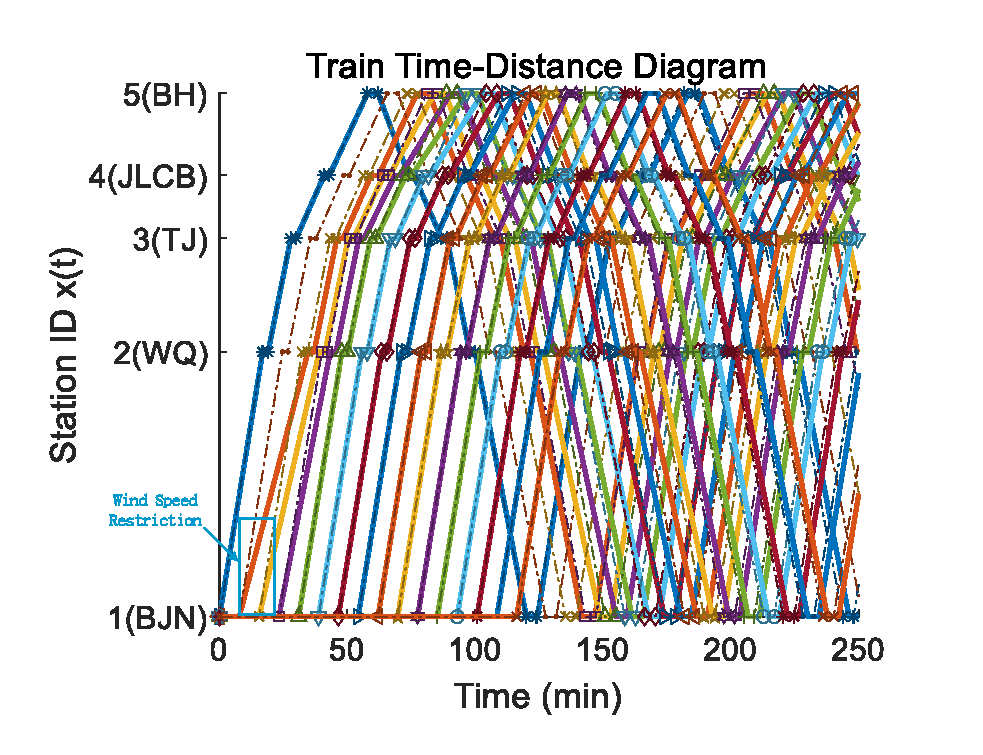
\includegraphics[width=\textwidth]{Img/Ch3/RunSit-no.pdf}
	\caption{名义时刻表（虚线）与FCFS策略下的实际时刻表（实线）}
	\label{fig:traingraphOriginalFCFS}
\end{figure}

\subsection{案例研究1（名义时刻表恢复）}
本案例中，向仿真系统引入小规模延误。在此类轻度扰动下，高速列车有能力恢复原始名义时刻表。因此可采用用于名义时刻表恢复的交通控制器（式(18)），其中参数 $g = -0.9$，$f = 0.7$。同时，我们在相同场景下也应用MIP方法进行实验。两种方法的结果如下所示。

\begin{figure}
	\centering
	\subfloat[所提实时自动交通控制器生成的重调度列车运行图（用于名义时刻表恢复）]{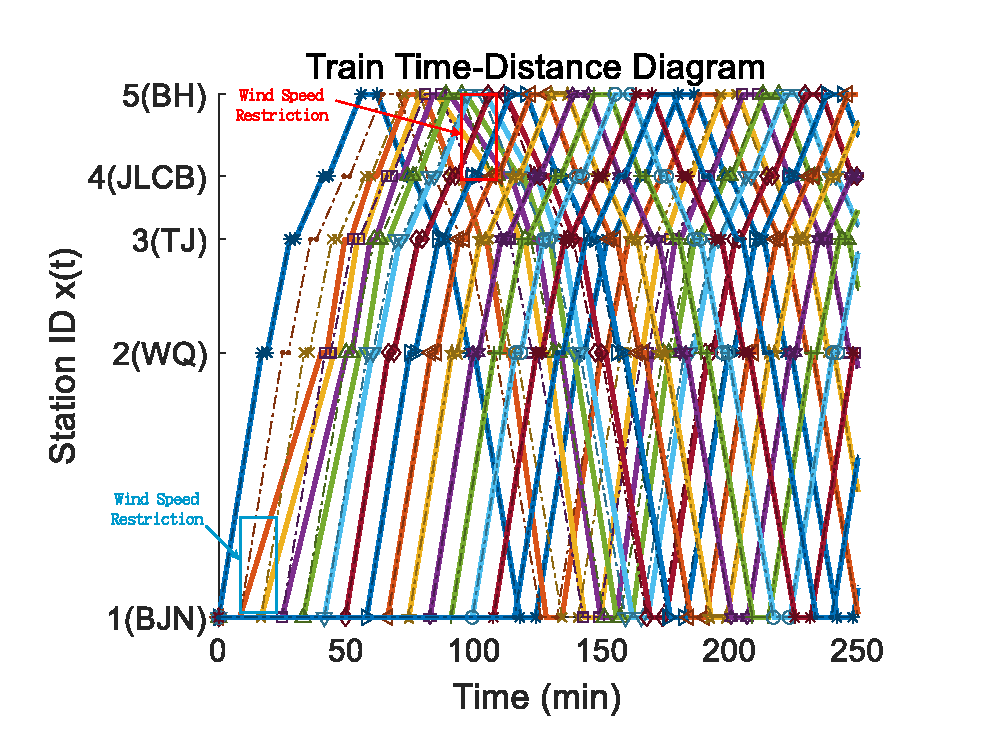
\includegraphics[width=\textwidth]{Img/Ch3/RunSit-with2.pdf}\label{fig:case1_subfig1}}
	\hfill
	\subfloat[MIP方法生成的重调度列车运行图]{\includegraphics[width=\textwidth]{Img/Ch3/Runsit-youhua2.pdf}\label{fig:case1_subfig2}}
	\caption{案例1中的闭环列车运行图}
	\label{fig:case1}
\end{figure}

\begin{figure}
	\centering
	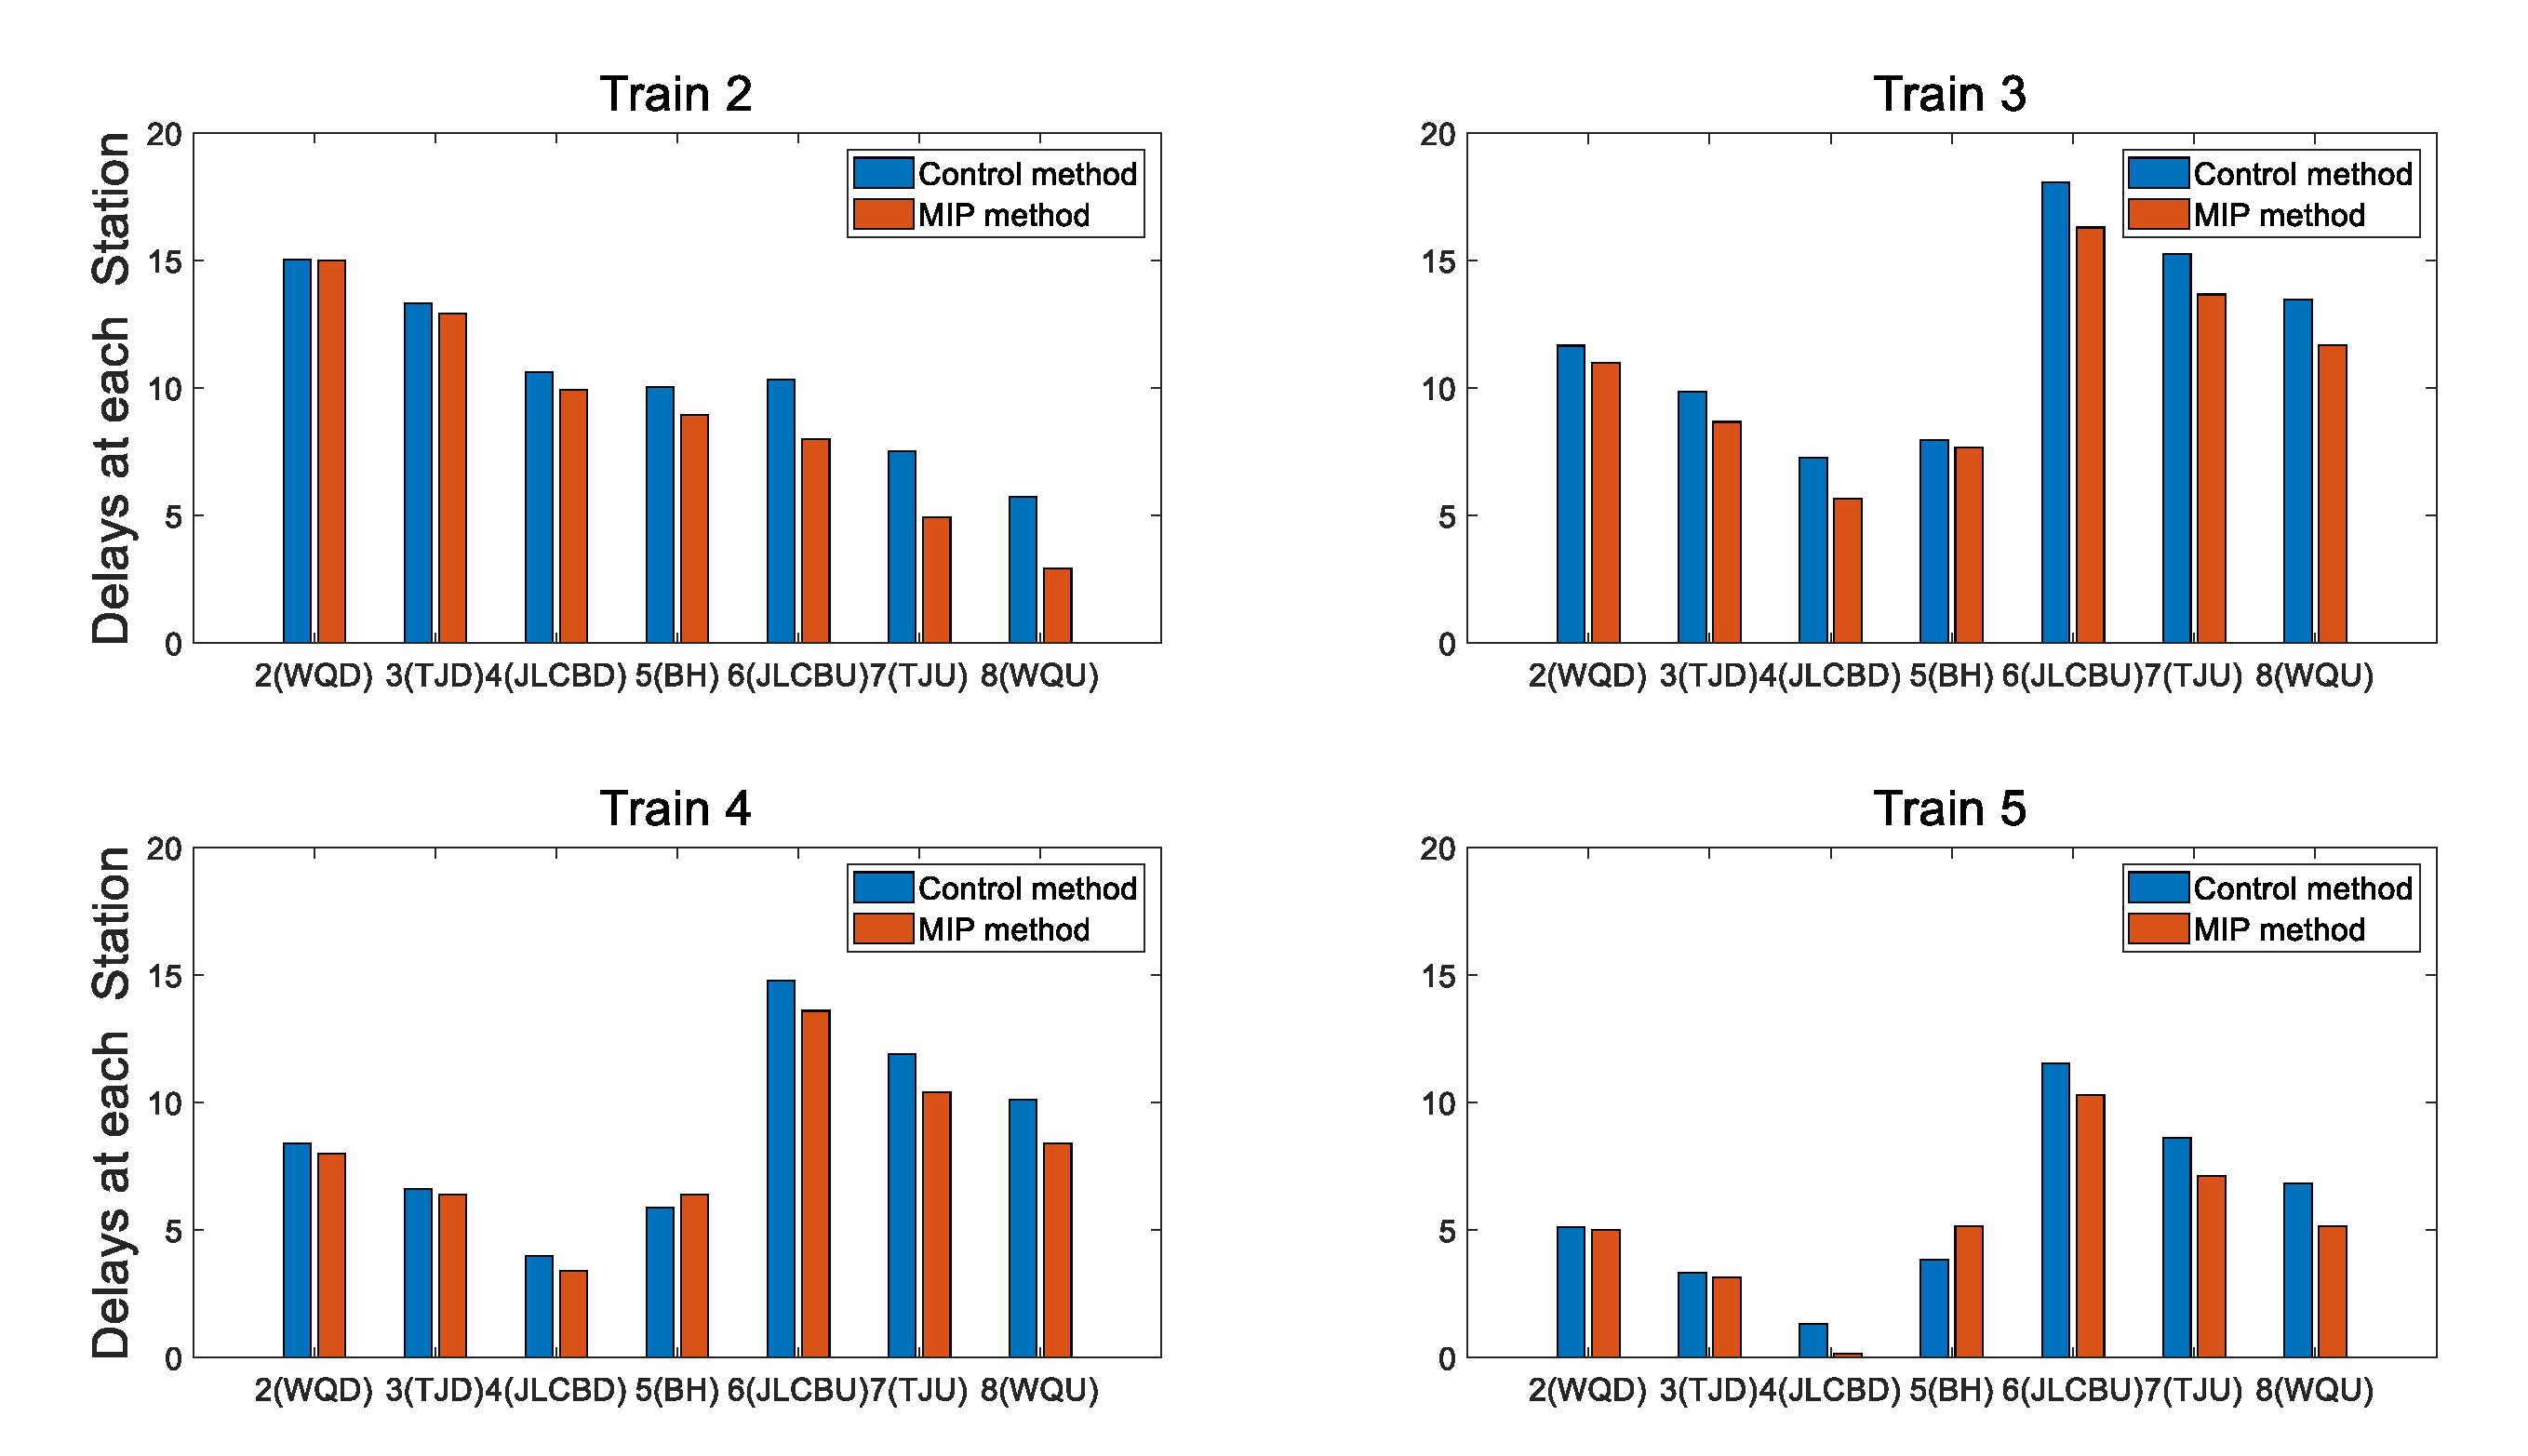
\includegraphics[width=\textwidth]{Img/Ch3/fourfig-youhua-controlwith.pdf}
	\caption{名义时刻表恢复控制器与MIP方法下列车2–5的出发延误演化图}
	\label{fig5:2_C-Obelt}
\end{figure}

本实验中引入了两次不同的小规模延误。图 \ref{fig:case1} 展示了所提交通控制器与MIP方法在列车时刻表恢复方面的结果，图 \ref{fig5:2_C-Obelt} 则展示了列车2–5在各站出发延误的演化过程。

如图 \ref{fig:case1_subfig1} 所示，针对列车2在车站1（BJN）至车站2（WQ）区间首次发生的15分钟运行延误，不仅列车2到达车站2时晚点15分钟，该延误还传播至后续列车3和4，使其分别产生11.6分钟和8.4分钟的出发延误。对于所提交通控制器，经过约8个车站后，列车2成功消除15分钟延误，按名义时刻表准点运行。由于列车3和4受此次主延误影响较小，其延误恢复速度相对较快。对于MIP方法，列车2在约7个车站后即恢复准点，列车3和4的延误则在约3个车站后基本消除。

第二次主延误发生在列车3从车站5（滨海，BH）驶向车站4（军粮城北，JLCB）的区间，此时第一次延误尚未完全消除。该事件导致列车3到达车站4时晚点16.8分钟，并进一步传播至后续列车4和5，使其分别产生13.6分钟和10.3分钟的出发延误。对于所提交通控制器，经过约5个车站后，列车3即可消除16.3分钟的延误并恢复名义时刻表运行；列车4和5因受影响较小，恢复更快。MIP方法则在约4个车站后使列车3恢复准点，列车4和5的延误也在约3个车站后基本消除。

从上述结果可见，在名义时刻表恢复控制器作用下，列车延误逐渐减小并收敛至零，其效果与MIP方法相当接近。两种方法在延误时间指标上的差距仅为6.1\%。

在最优控制理论中，通常通过线性二次调节器（LQR）或控制器匹配技术，寻找与标准代价函数最优解等效的反馈控制器。由于所提控制器的代价函数同时考虑了延误时间、发车间隔和控制量，而MIP方法未显式约束控制量，因此其性能略优于所提方法。

然而，MIP方法的平均计算时间为56秒，更重要的是，它无法满足城际高速铁路对**实时调度**的需求。相比之下，所提交通控制器的平均计算时间仅为0.006秒，完全满足实时性要求。因此，在小规模延误场景下，用于名义时刻表恢复的交通控制器兼具高效性与实时性。

\subsection{案例研究2（维持规律发车间隔）}
本实验中，列车2和列车3在运行途中遭遇线路事故，被迫在区间内停车。其余列车在接收到故障信息后出发时间均被推迟，导致严重延误——列车2在车站2处晚点达50分钟。在此场景下，列车难以恢复名义时刻表，因此采用所提交通控制器以维持**规律发车间隔**。MIP方法仍保持不变。图 \ref{fig:case2} 展示了两种方法在维持列车均匀发车方面的结果：图 \ref{fig:case2_subfig1} 为所提控制器结果，图 \ref{fig:case2_subfig2} 为MIP方法结果。图 \ref{fig5:4_C-Obelt} 则展示了各站列车发车间隔方差的演化过程。

如图 \ref{fig:case2_subfig1} 所示，与案例1类似，列车2在车站1（BJN）至车站2（WQ）区间遭遇50分钟的大规模运行延误，导致后续13列列车均产生不同程度的延误。但本案例关注的是在严重扰动下如何维持**规律发车间隔**。由图 \ref{fig5:4_C-Obelt} 可见，延误对后续列车的传播被有效抑制。对于用于规律发车间隔的交通控制器（式(33)），经过约11个车站后，列车发车间隔方差可降至约10，列车群基本实现规律发车。MIP方法则需约15个车站才能达到类似效果，恢复速度较慢。

由此可见，在规律发车间隔控制器作用下，列车发车间隔方差逐渐减小并趋于稳定，其效果与MIP方法相近，两者在发车间隔方差指标上的差距仅为2.5\%。同样，由于所提控制器与MIP的代价函数不同，MIP性能略优。但与案例1类似，MIP方法的平均计算时间高达65秒，无法满足实时调度需求；而所提控制器平均仅需0.005秒，具备良好的实时性。因此，在严重延误场景下，用于维持规律发车间隔的交通控制器同样高效且实时。

\begin{figure}
	\centering
	\subfloat[所提交通控制器（用于规律发车间隔）生成的列车运行图]{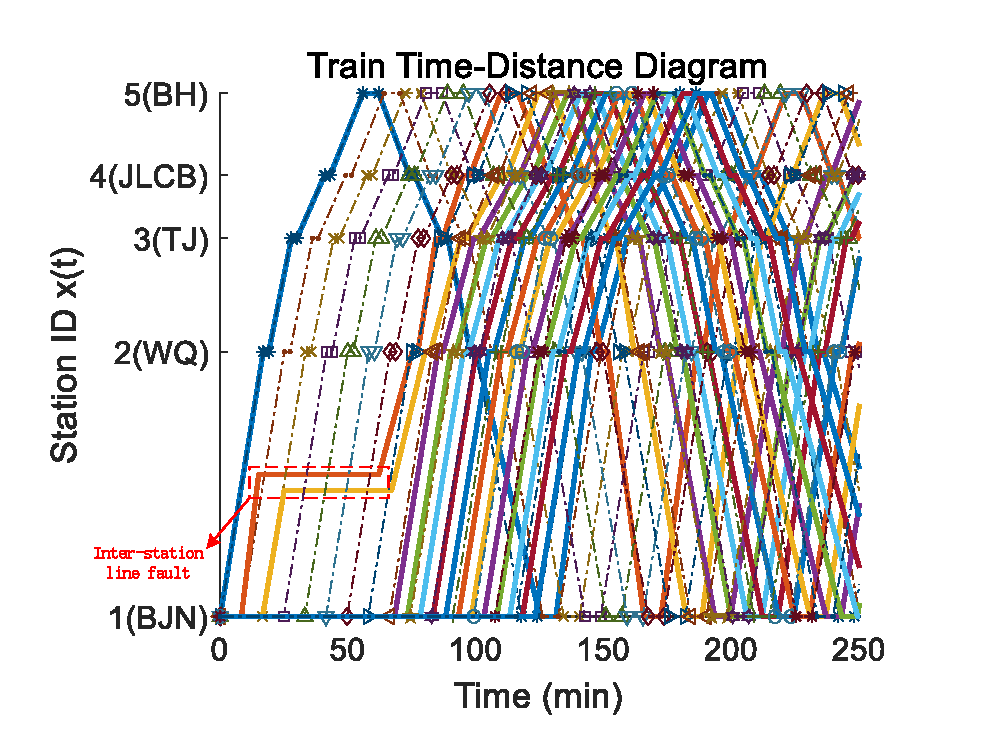
\includegraphics[width=\textwidth]{Img/Ch3/RunSit-nowithbig.pdf}\label{fig:case2_subfig1}}
	\hfill
	\subfloat[MIP方法生成的闭环列车运行图]{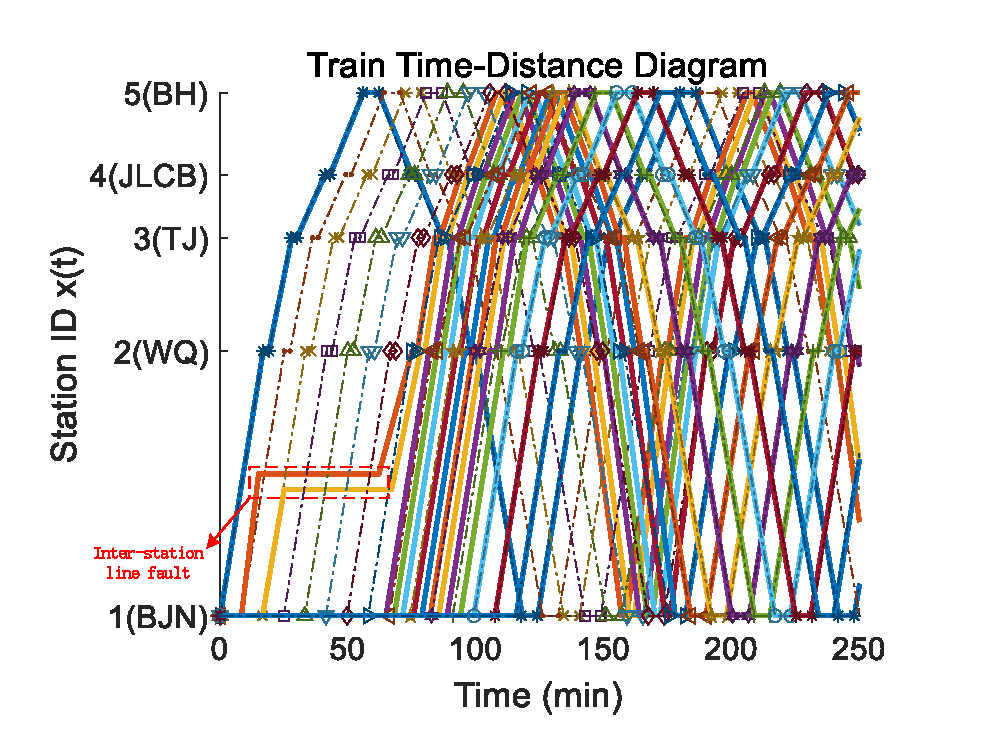
\includegraphics[width=\textwidth]{Img/Ch3/RunSit-mpcbig.pdf}\label{fig:case2_subfig2}}
	\caption{案例2中的闭环列车运行图}
	\label{fig:case2}
\end{figure}

\begin{figure}
	\centering
	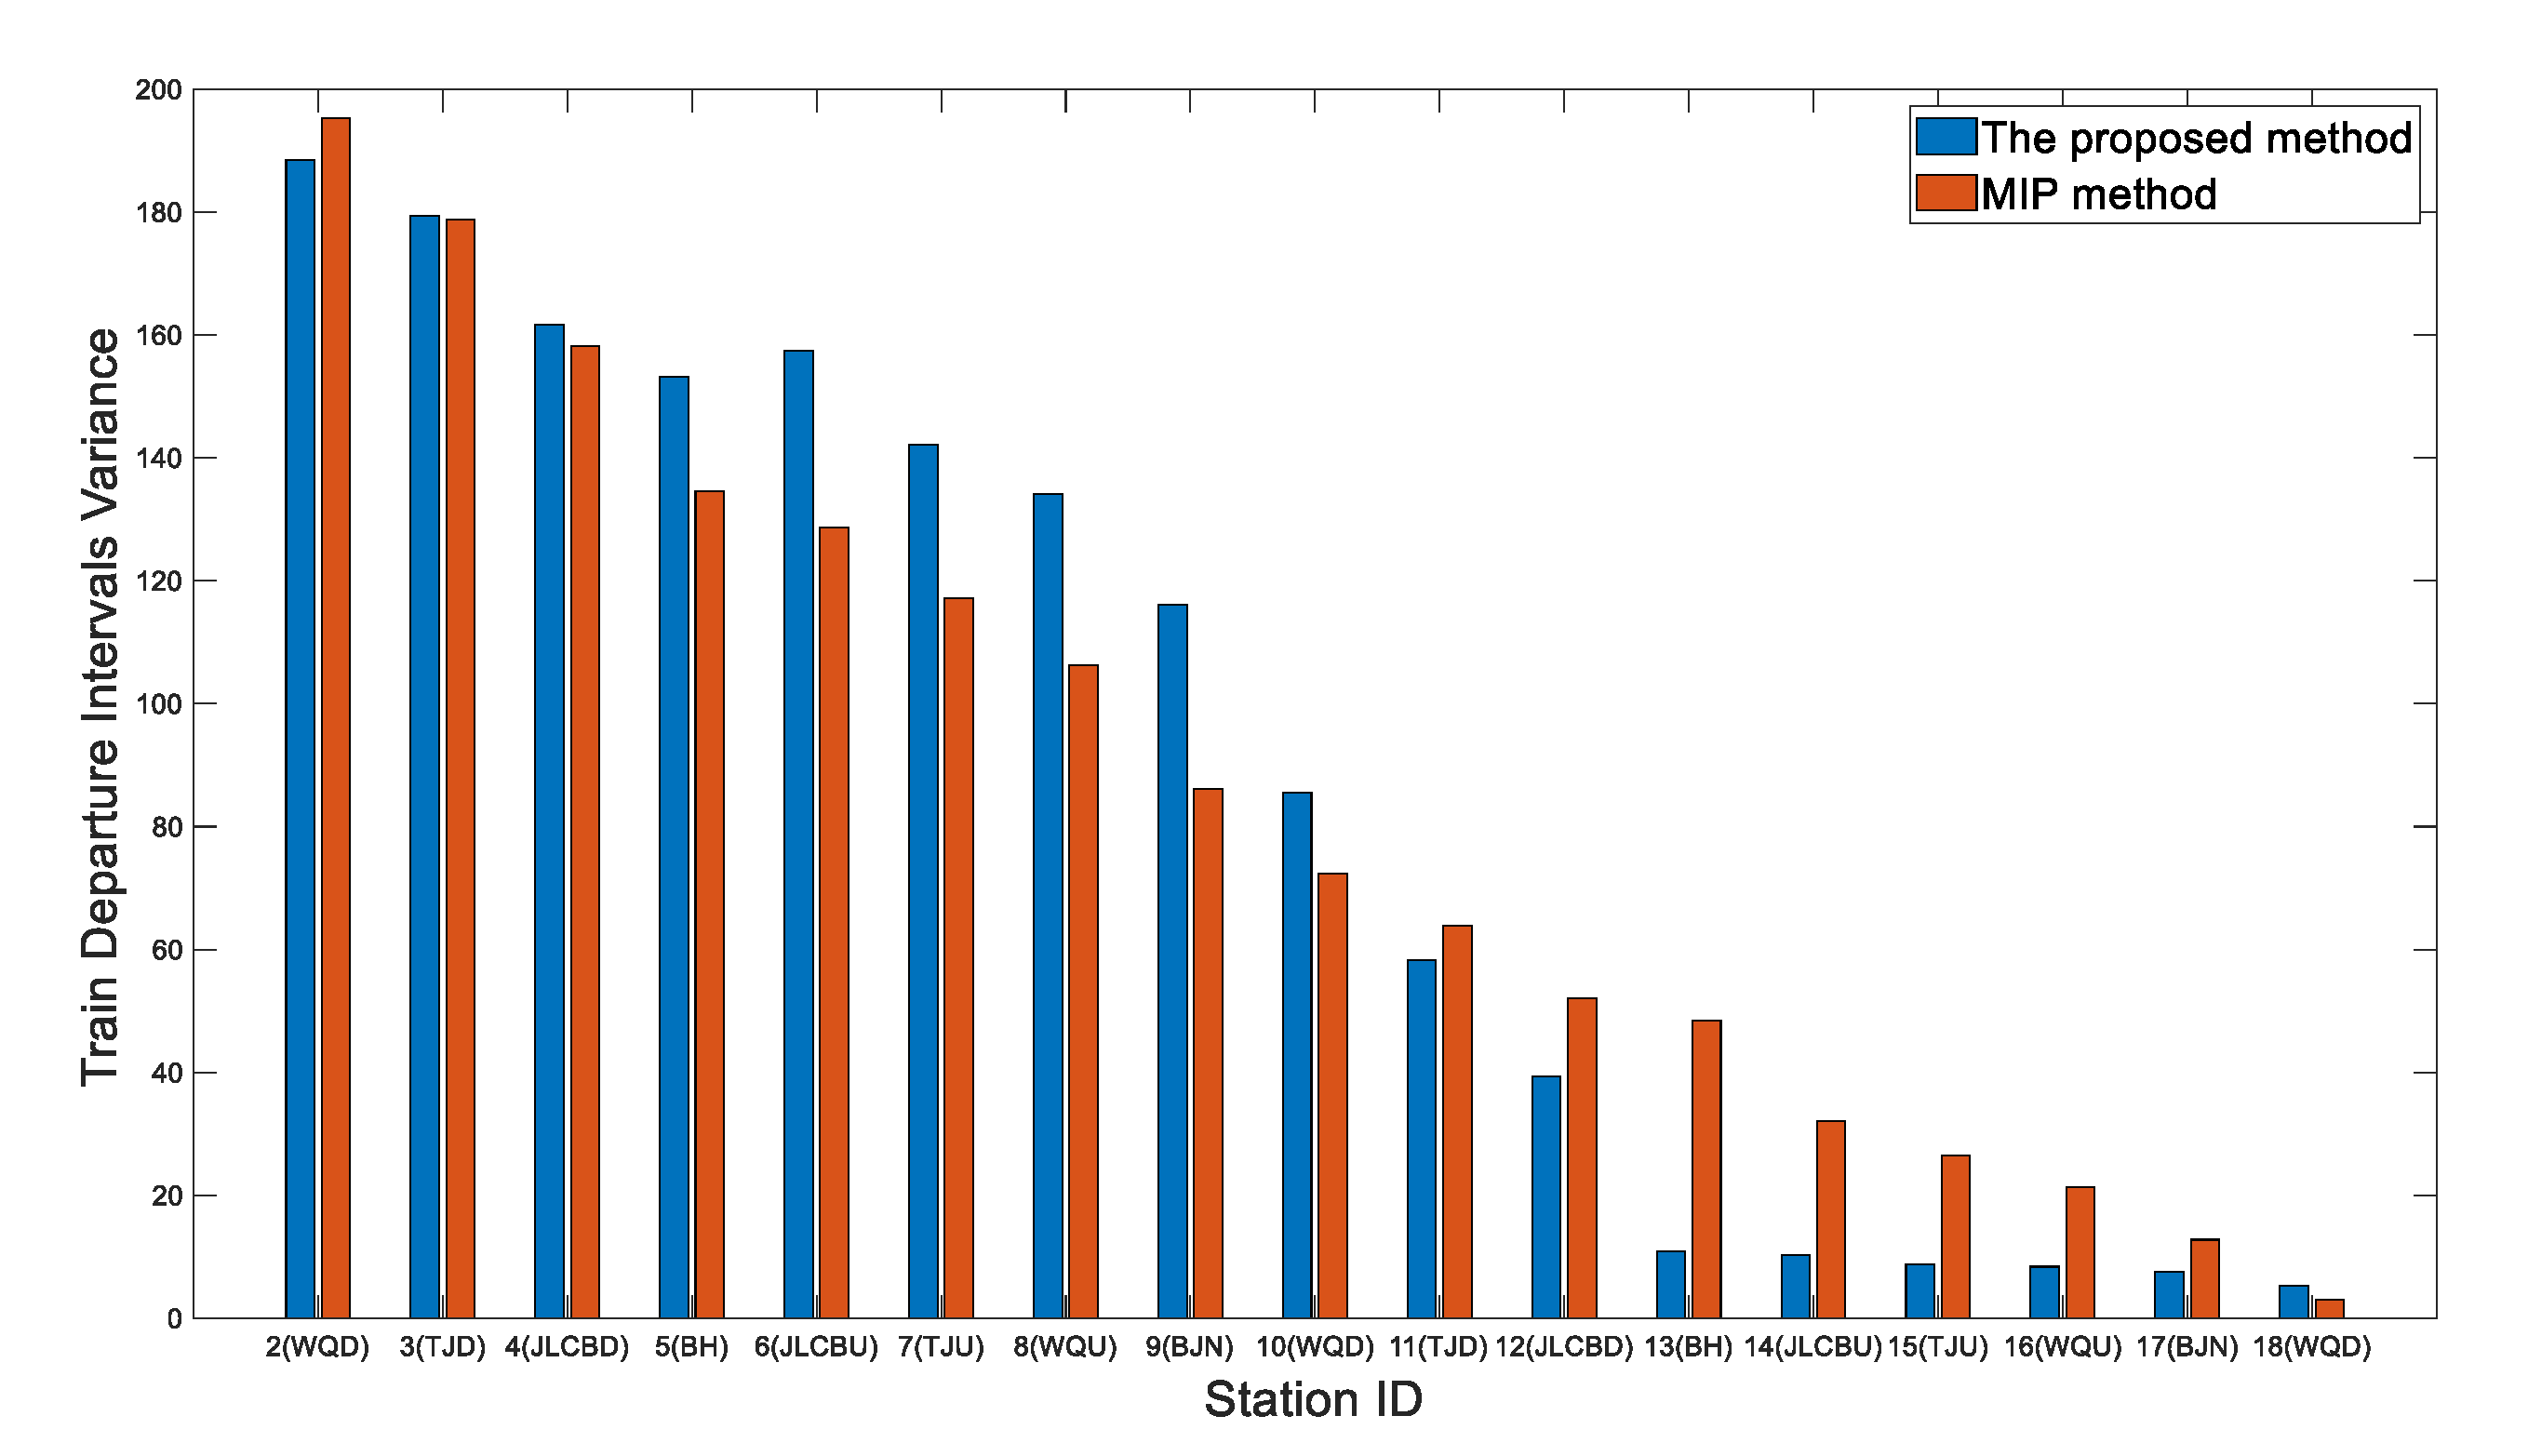
\includegraphics[width=\textwidth]{Img/Ch3/intervalVariance.pdf}
	\caption{规律发车间隔控制器与MIP方法下发车间隔方差演化图}
	\label{fig5:4_C-Obelt}
\end{figure}

\subsection{计算时间分析}
为更全面地评估所提方法与MIP方法的计算效率，我们选取多个不同规模的场景，分别测试两种控制器（名义时刻表恢复与规律发车间隔）及MIP方法的计算时间，如下表所示。线路实际车站数为8个，但由于列车循环运行，虚拟车站数等于列车实际经过的车站总数。

\begin{table}
	\centering
	\caption{小规模延误下不同场景的计算时间对比（单位：秒）}
	\begin{tabular}{cccc}
		\hline
		列车数 & 车站数 & 名义时刻表恢复控制器 & MIP方法 \\
		\hline
		12 & 41 & 0.000062 & 31.42 \\
		13 & 44 & 0.000065 & 38.50 \\
		14 & 48 & 0.000067 & 48.66 \\
		15 & 51 & 0.000057 & 56.87 \\
		16 & 54 & 0.000065 & 78.64 \\
		17 & 57 & 0.000062 & 89.27 \\
		18 & 61 & 0.000061 & 104.44 \\
		19 & 64 & 0.000058 & 122.73 \\
		20 & 67 & 0.000067 & 140.19 \\
		\hline
	\end{tabular}
\end{table}

\begin{table}
	\centering
	\caption{严重延误下不同场景的计算时间对比（单位：秒）}
	\begin{tabular}{cccc}
		\hline
		列车数 & 车站数 & 发车间隔调节控制器 & MIP方法 \\
		\hline
		12 & 41 & 0.000061 & 35.17 \\
		13 & 44 & 0.000063 & 42.41 \\
		14 & 48 & 0.000064 & 52.17 \\
		15 & 51 & 0.000060 & 65.74 \\
		16 & 54 & 0.000059 & 79.99 \\
		17 & 57 & 0.000068 & 93.08 \\
		18 & 61 & 0.000057 & 109.86 \\
		19 & 64 & 0.000065 & 129.65 \\
		20 & 67 & 0.000063 & 146.68 \\
		\hline
	\end{tabular}
\end{table}

从表2与表3可见，尽管MIP方法在小规模延误下的计算时间短于严重延误场景，但其耗时仍远高于所提控制方法。更重要的是，两种所提控制器的计算时间**几乎不随问题规模增大而显著增加**。这一特性使其非常适合未来高密度、高速度的城际铁路发展趋势。

\section{本章小节}
本章针对城际高速铁路系统，构建了适用于多列车运行的状态空间动态模型，并根据扰动程度的不同，分别提出了面向轻度延误与严重延误的两种模型变体。在此基础上，设计了两类状态反馈自动重调度控制器：一是在轻度延误（如大风限速）场景下实现名义时刻表的快速恢复；二是在严重延误（如区间故障）场景下维持列车发车的规律性间隔。通过基于京津城际高速铁路的实际数据仿真验证，所提方法在两类典型扰动场景下均能有效抑制延误传播，保障系统运行稳定性。

与传统的混合整数规划（MIP）方法相比，本文所提控制器在性能上仅分别相差6.1\%\,和\,2.5\%，而计算时间从数十秒级大幅降低至微秒级（平均约0.006秒），显著满足高速铁路实时调度的需求。结果表明，该反馈控制策略在保持近似最优调度效果的同时，具备极高的计算效率与工程实用性，为高密度城际铁路网络的智能化、实时化调度提供了高效可行的技术路径。

